% =====================================================================
%  Inventário de figuras — fonte OpenAlex (IA nas Humanidades, internacional)
%  Paralelo a inventario_figuras_capes.md (fontes CAPES/SciELO).
%  Trecho pronto para inserir na tese (\input ou copiar). Requer \usepackage{graphicx}.
%  Figuras 01–09 geradas por figuras_openalex.py e figuras_openalex_mapa.py;
%  figuras 10–15 (temáticas) por figuras_openalex_temas.py (pasta figuras/).
%  Números: ver docs/decisoes_metodologicas.md, bloco IV (fonte canônica).
%
%  Convenções (idênticas às do inventario_figuras_capes.md):
%   - \label segue o padrão fig:openalex_NN_descritor (autoref/Cref).
%   - \fonte{...} é o comando comum em teses brasileiras (abnTeX2/ABNT);
%     se o seu template não o definir, troque por \source{}, \floatfoot{}
%     ou similar conforme o padrão do PPGAS-USP.
%   - largura padrão 0.95\linewidth — ajuste conforme o layout.
% =====================================================================

\subsection{A produção de IA nas Humanidades em perspectiva internacional (OpenAlex)}

Para situar o caso brasileiro num horizonte global, recorremos a uma terceira
fonte, o \textit{OpenAlex} --- catálogo aberto de cerca de 250 milhões de obras
acadêmicas. Diferentemente da CAPES e do SciELO, restritos ao Brasil,
o OpenAlex permite comparar países e disciplinas. Adotamos como recorte de
``Humanidades'' a união dos \textit{fields} \textit{Arts and Humanities},
\textit{Psychology} e \textit{Social Sciences} (na taxonomia do OpenAlex,
herdada da Scopus/ASJC), de modo a espelhar a grande área ``Ciências Humanas''
da CAPES, que igualmente abriga a Psicologia. A janela analisada é
2016--2024, e a identificação de obras de IA combina o conceito
\textit{Artificial intelligence} do OpenAlex com a mesma régua de palavras-chave
empregada nas demais fontes (\texttt{utils.classificar\_subcampos}).

É preciso, de saída, distinguir duas definições de ``IA'' que produzem
magnitudes distintas sobre a \emph{mesma} base. Pela tag conceitual do OpenAlex,
o Brasil registra 9.996 obras de IA nas Humanidades no período; pela régua de
palavra-chave --- a mesma que sustenta os números da CAPES e do
SciELO ---, apenas 849 obras únicas mencionam, de fato, vocabulário de IA em
título ou resumo. Ou seja, somente cerca de 8,5\% das obras que o classificador
do OpenAlex sinaliza como ``IA'' contêm esse vocabulário explícito --- diferença
atribuível tanto à generosidade do conceito algorítmico quanto à ausência de
resumo em parte das obras. As comparações internacionais de volume e penetração
(Figuras~\ref{fig:openalex_01_ranking_paises},
\ref{fig:openalex_02_taxa_interna_paises}
e~\ref{fig:openalex_03_brasil_temporal}) empregam a definição por conceito, mais
inclusiva e uniforme entre países; a análise de subcampos
(Figura~\ref{fig:openalex_04_subcampos_3bases}) emprega a régua de
palavra-chave, comparável às outras fontes.

% ---------------------------------------------------------------------
\begin{figure}[htbp]
  \centering
  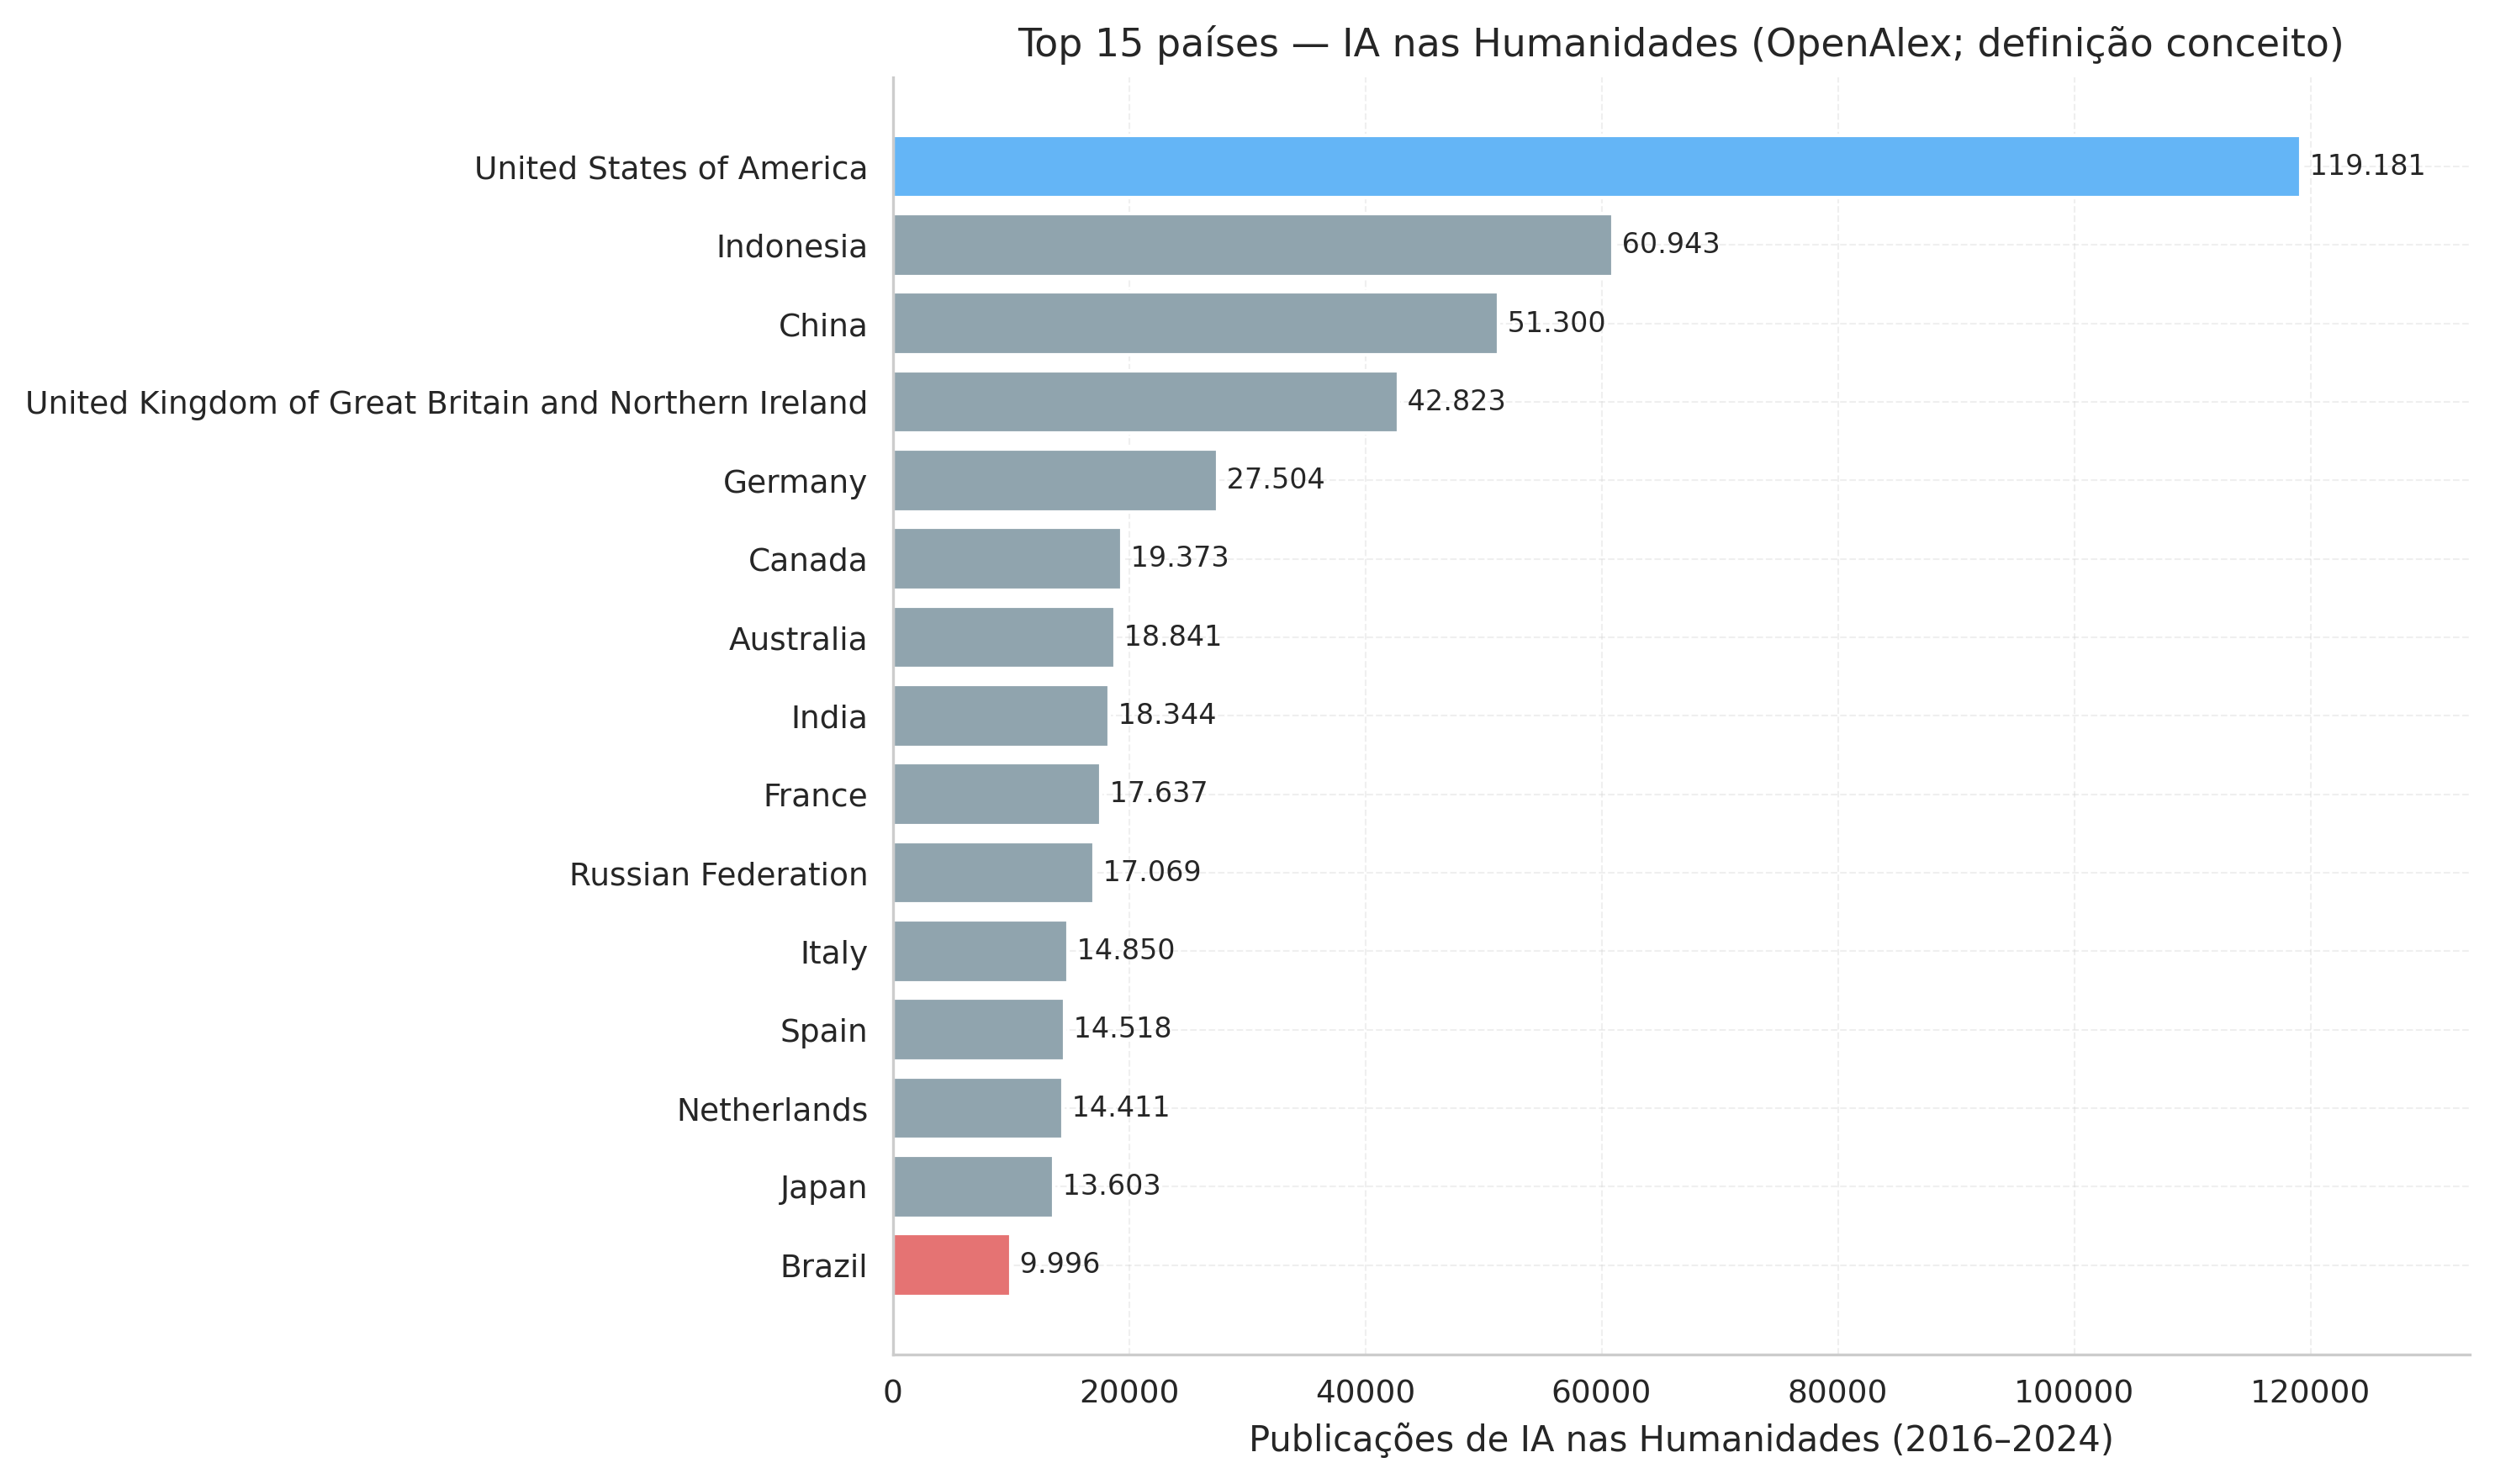
\includegraphics[width=0.95\linewidth]{figuras/openalex_01_ranking_paises.png}
  \caption{Os quinze maiores produtores de publicações sobre inteligência
  artificial na grande área de Humanidades, 2016--2024, segundo o OpenAlex
  (definição por conceito). O Brasil, destacado em vermelho, ocupa a
  14.\textsuperscript{a} posição mundial em volume absoluto (9.996 obras),
  atrás de produtores como Estados Unidos (cerca de 60,9 mil), China (51,3 mil),
  Reino Unido (42,8 mil) e Alemanha (27,5 mil).}
  \label{fig:openalex_01_ranking_paises}
  \fonte{Elaboração própria a partir do OpenAlex (2016--2024).}
\end{figure}

A Figura~\ref{fig:openalex_01_ranking_paises} evidencia forte concentração
geográfica: os Estados Unidos (cerca de 60,9 mil obras) e a China (51,3 mil)
lideram com larga vantagem, seguidos pelo Reino Unido (42,8 mil) e pela Alemanha
(27,5 mil). Cabe notar uma inversão reveladora: nas estatísticas de IA \emph{em
todas as áreas} --- como as do \textit{Country Activity Tracker} do CSET ---, a
China supera os Estados Unidos em volume; quando o recorte é a Humanidades, os
Estados Unidos retomam a dianteira. A interseção entre IA e Humanidades tem,
portanto, uma geografia própria, distinta da IA tomada em sentido amplo. O
Brasil, com 9.996 obras, figura em 14.\textsuperscript{o} lugar --- presença não
desprezível em volume absoluto, mas que, como se verá, oculta uma baixíssima
penetração relativa.

% ---------------------------------------------------------------------
\begin{figure}[htbp]
  \centering
  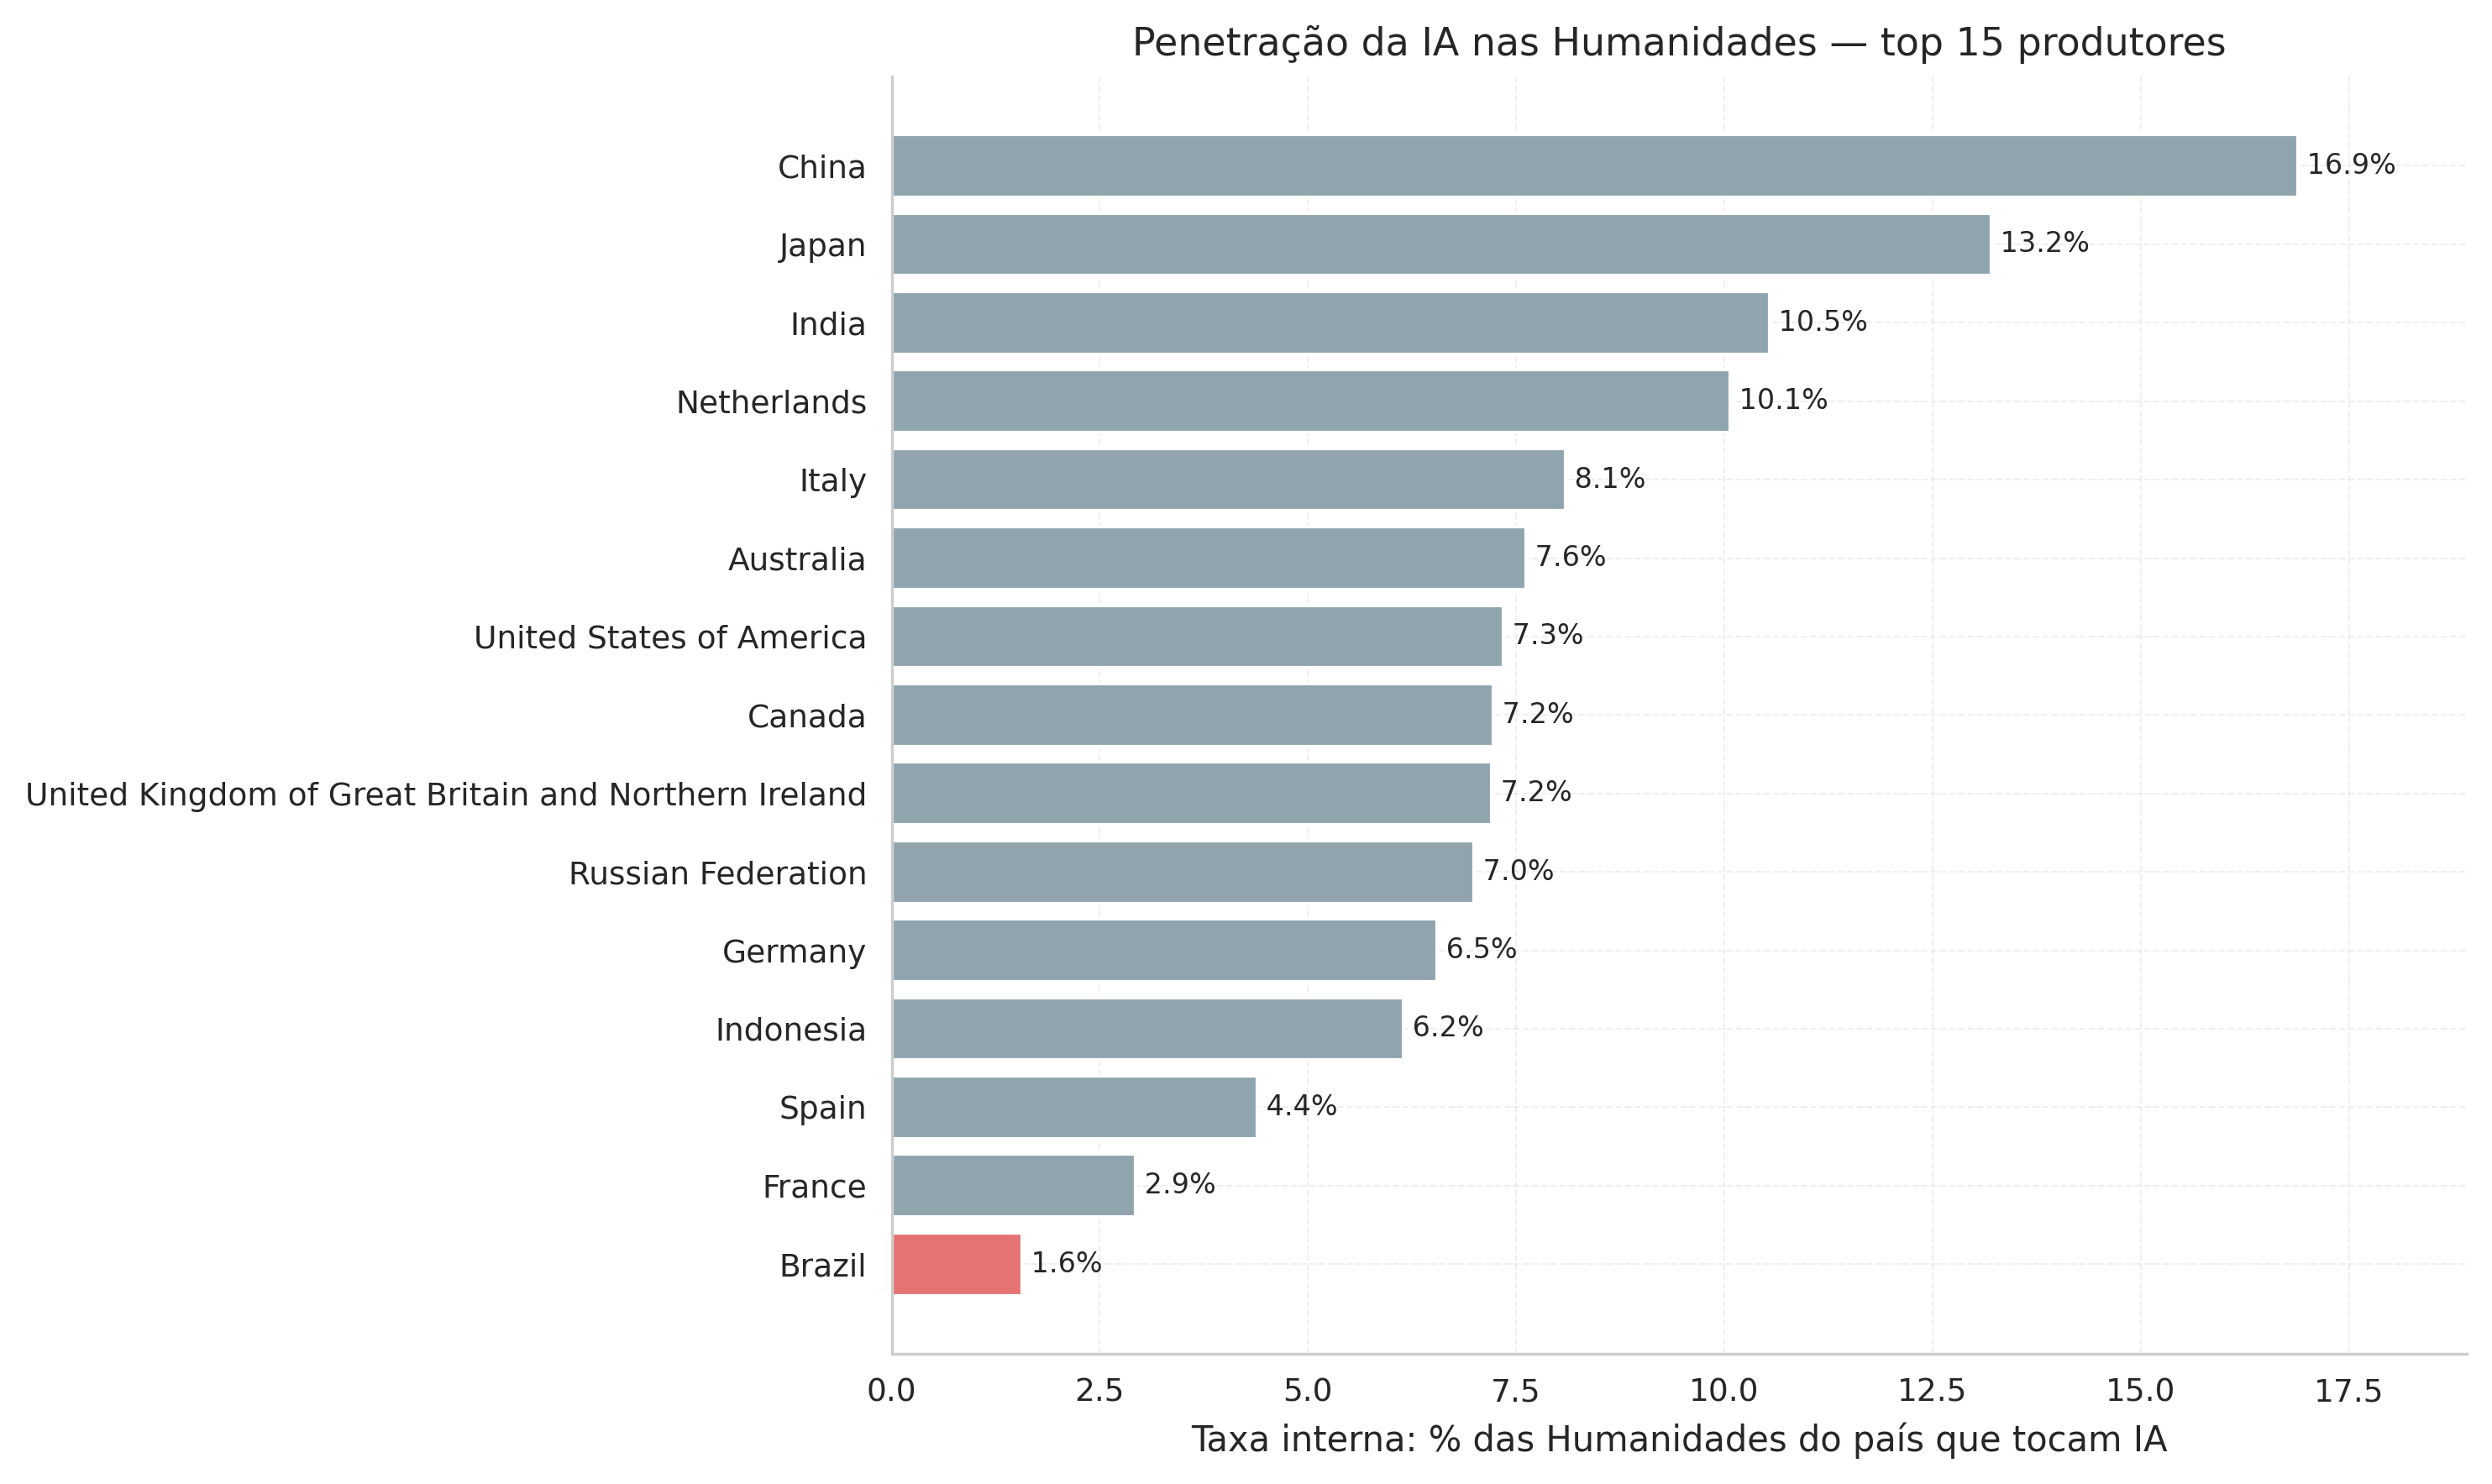
\includegraphics[width=0.95\linewidth]{figuras/openalex_02_taxa_interna_paises.png}
  \caption{Taxa interna --- proporção das publicações de Humanidades de cada país
  que tocam o campo da IA --- entre os quinze maiores produtores, 2016--2024.
  Apesar do volume, o Brasil (destacado em vermelho) apresenta a menor taxa do
  grupo (1,57\%), contra 16,89\% da China, 13,20\% do Japão e 6,15\% dos Estados
  Unidos.}
  \label{fig:openalex_02_taxa_interna_paises}
  \fonte{Elaboração própria a partir do OpenAlex (2016--2024).}
\end{figure}

A leitura por \emph{taxa interna} --- isto é, a fração das Humanidades de cada
país que dialoga com a IA --- altera radicalmente o quadro
(Figura~\ref{fig:openalex_02_taxa_interna_paises}). A China lidera a penetração
com 16,89\%, seguida por Japão (13,20\%), Índia (10,54\%) e Países Baixos
(10,07\%); os Estados Unidos, primeiros em volume, exibem penetração
intermediária (6,15\%). O Brasil ocupa o \emph{último} lugar entre os quinze
maiores produtores, com apenas 1,57\%. O dado é tanto mais expressivo quando se
observa que o Brasil possui o segundo maior \emph{universo} de Humanidades do
conjunto (636.607 obras, atrás apenas dos Estados Unidos): não se trata, pois, de
um país que produz pouco em Humanidades, mas de um país cuja vasta produção
humanística pouco se conecta à IA. Esse achado replica, em escala internacional,
a ``marginalidade'' já diagnosticada na CAPES (0,67\% das defesas de Humanas
tocam a IA) e no SciELO, conferindo-lhe robustez por triangulação entre fontes
independentes.

% ---------------------------------------------------------------------
\begin{figure}[htbp]
  \centering
  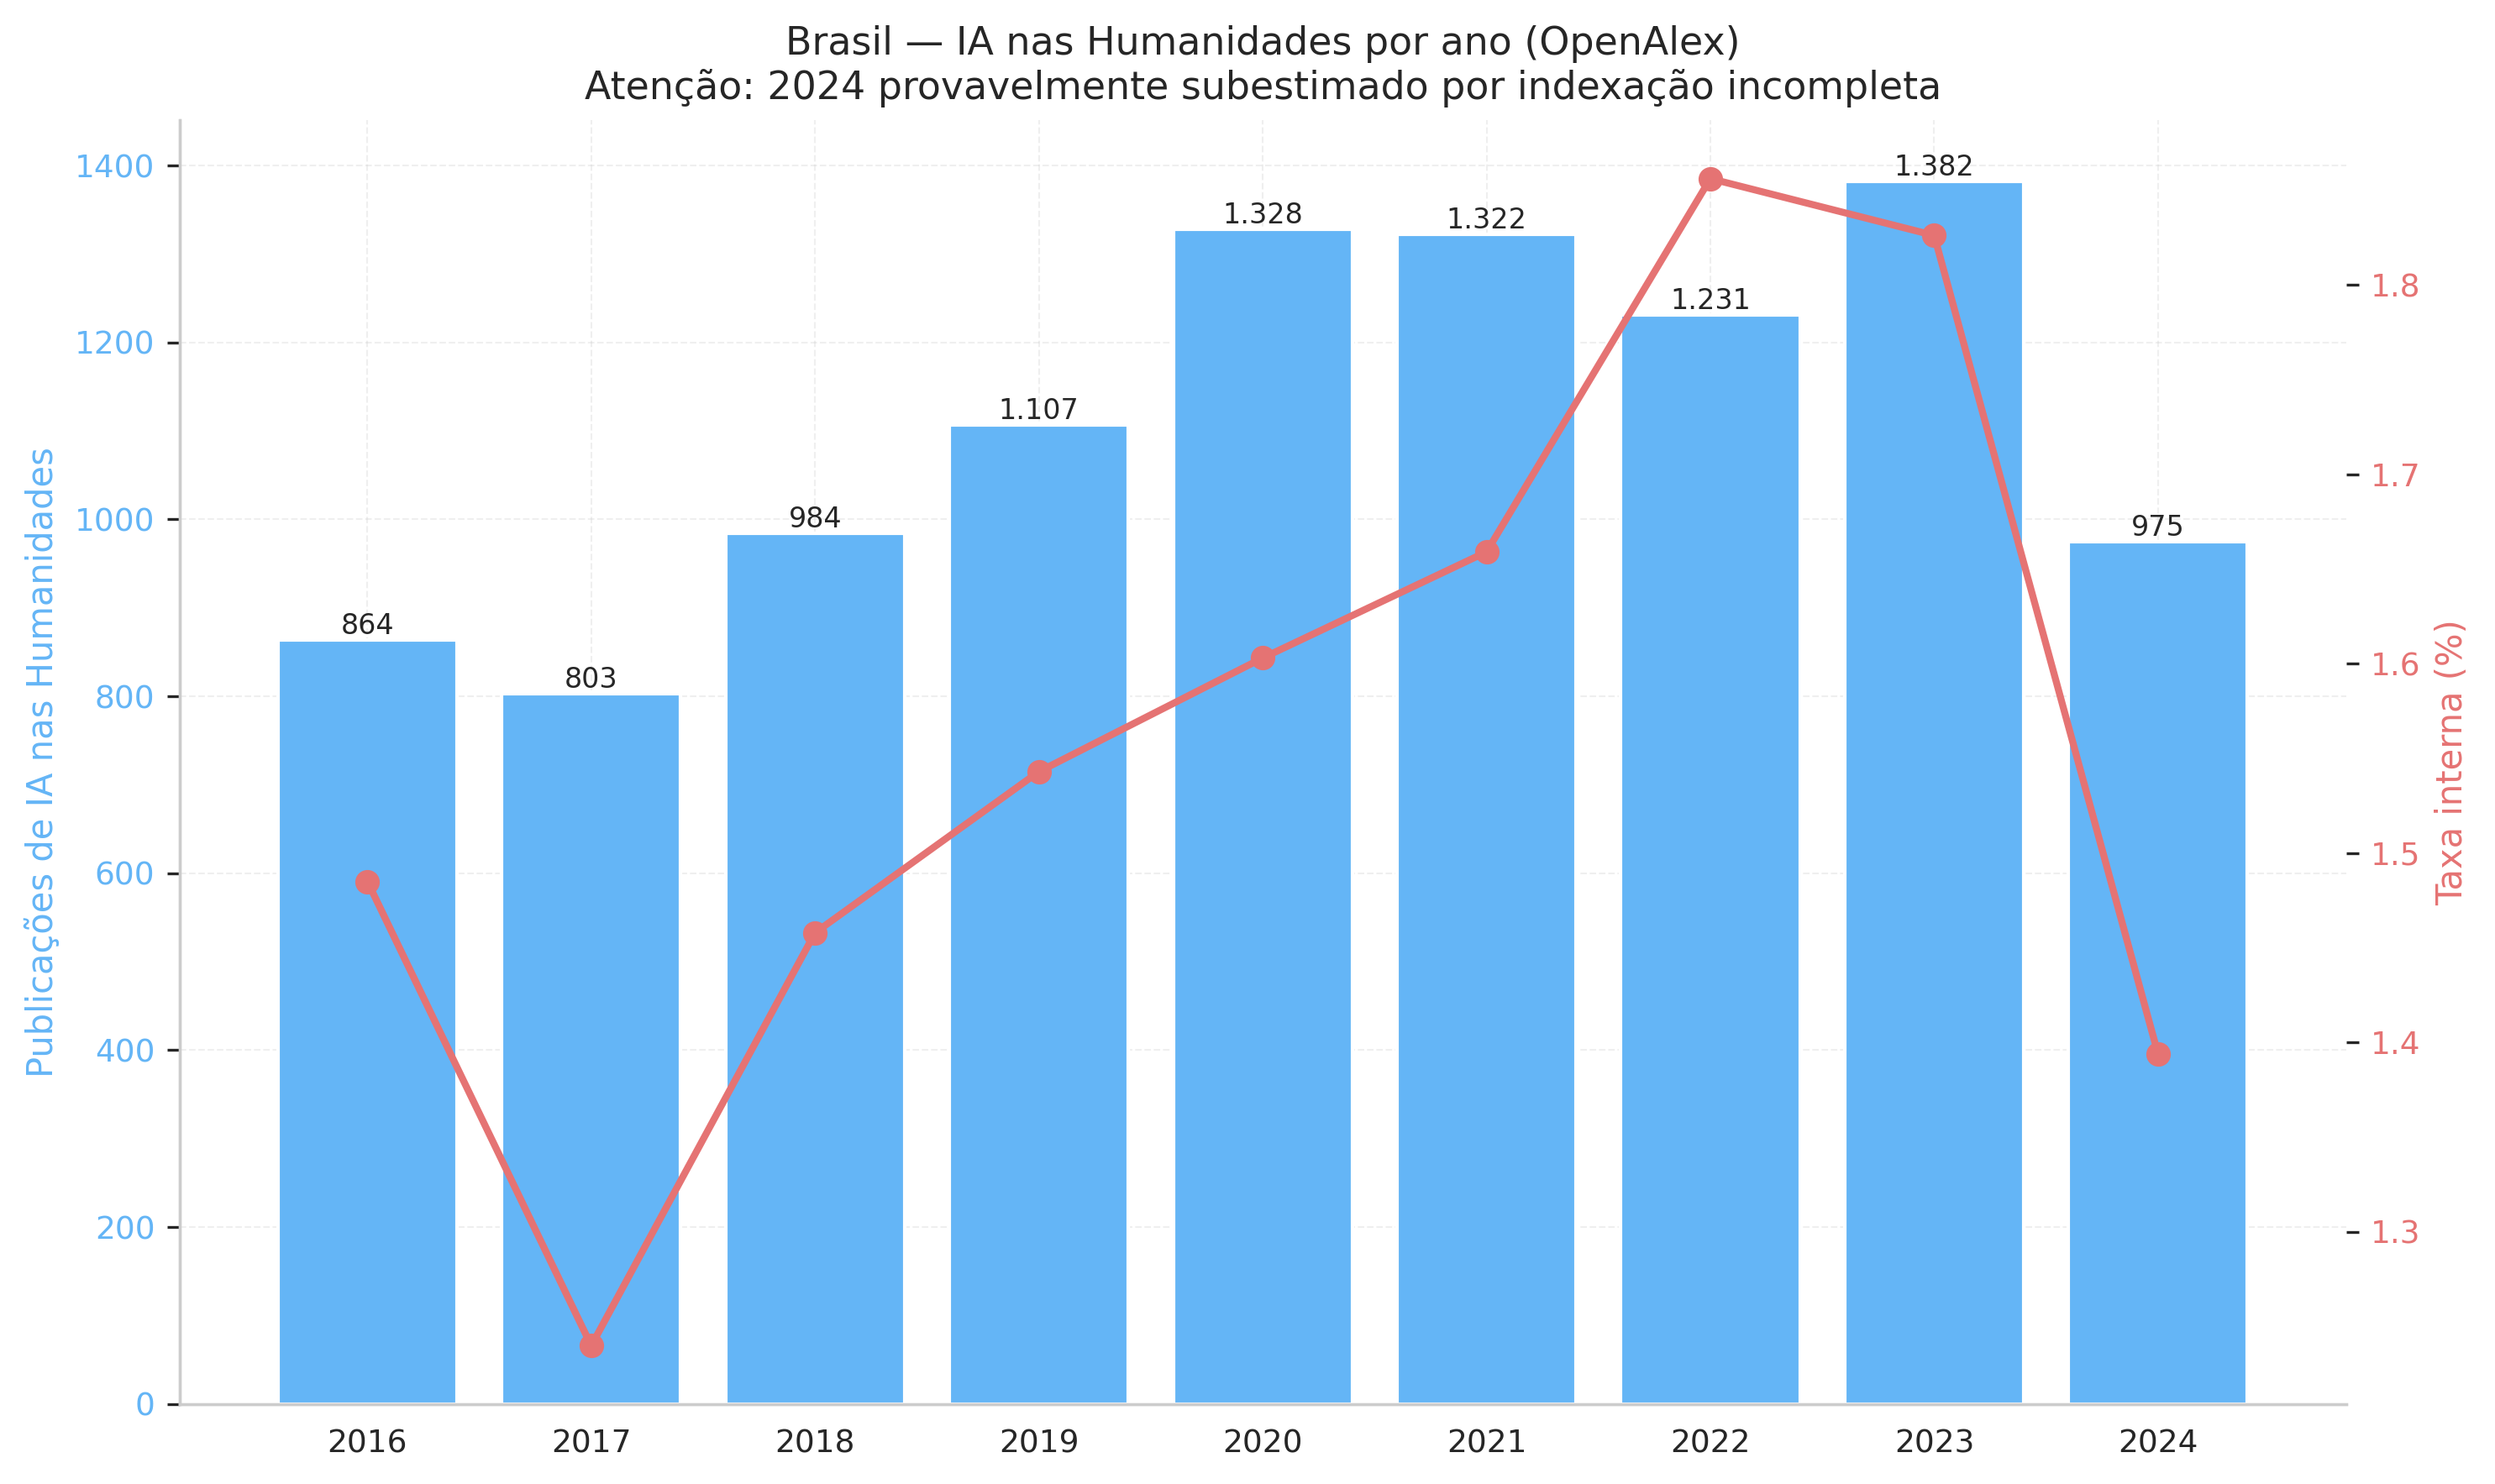
\includegraphics[width=0.95\linewidth]{figuras/openalex_03_brasil_temporal.png}
  \caption{Brasil: volume anual de publicações de IA nas Humanidades (barras) e
  taxa interna (linha), 2016--2024. O volume cresce de 864 obras (2016) a 1.382
  (2023), enquanto a taxa interna permanece estável entre 1,2\% e 1,9\%. A
  retração de 2024 deve-se, muito provavelmente, à indexação ainda incompleta do
  ano no OpenAlex, não a um declínio real.}
  \label{fig:openalex_03_brasil_temporal}
  \fonte{Elaboração própria a partir do OpenAlex (2016--2024).}
\end{figure}

A trajetória temporal brasileira (Figura~\ref{fig:openalex_03_brasil_temporal})
mostra crescimento sustentado entre 2016 (864 obras) e 2023 (1.382 obras),
acompanhado de uma taxa interna que oscila entre 1,2\% e 1,9\%, com pico em 2022
(1,86\%). A aparente queda de 2024 (975 obras) deve ser lida com cautela: o
OpenAlex segue indexando publicações do ano mais recente, de modo que o valor é
quase certamente subestimado --- limitação análoga à observada na própria base
do CSET. O traço marcante não é a flutuação anual, mas a \emph{estabilidade em
patamar baixo} da taxa interna: ainda que o volume cresça, a fração das
Humanidades brasileiras que incorpora a IA permanece estagnada em torno de
1,5\%, o que sugere expansão concentrada em poucos nichos, e não difusão ampla
pelo campo.

% ---------------------------------------------------------------------
\begin{figure}[htbp]
  \centering
  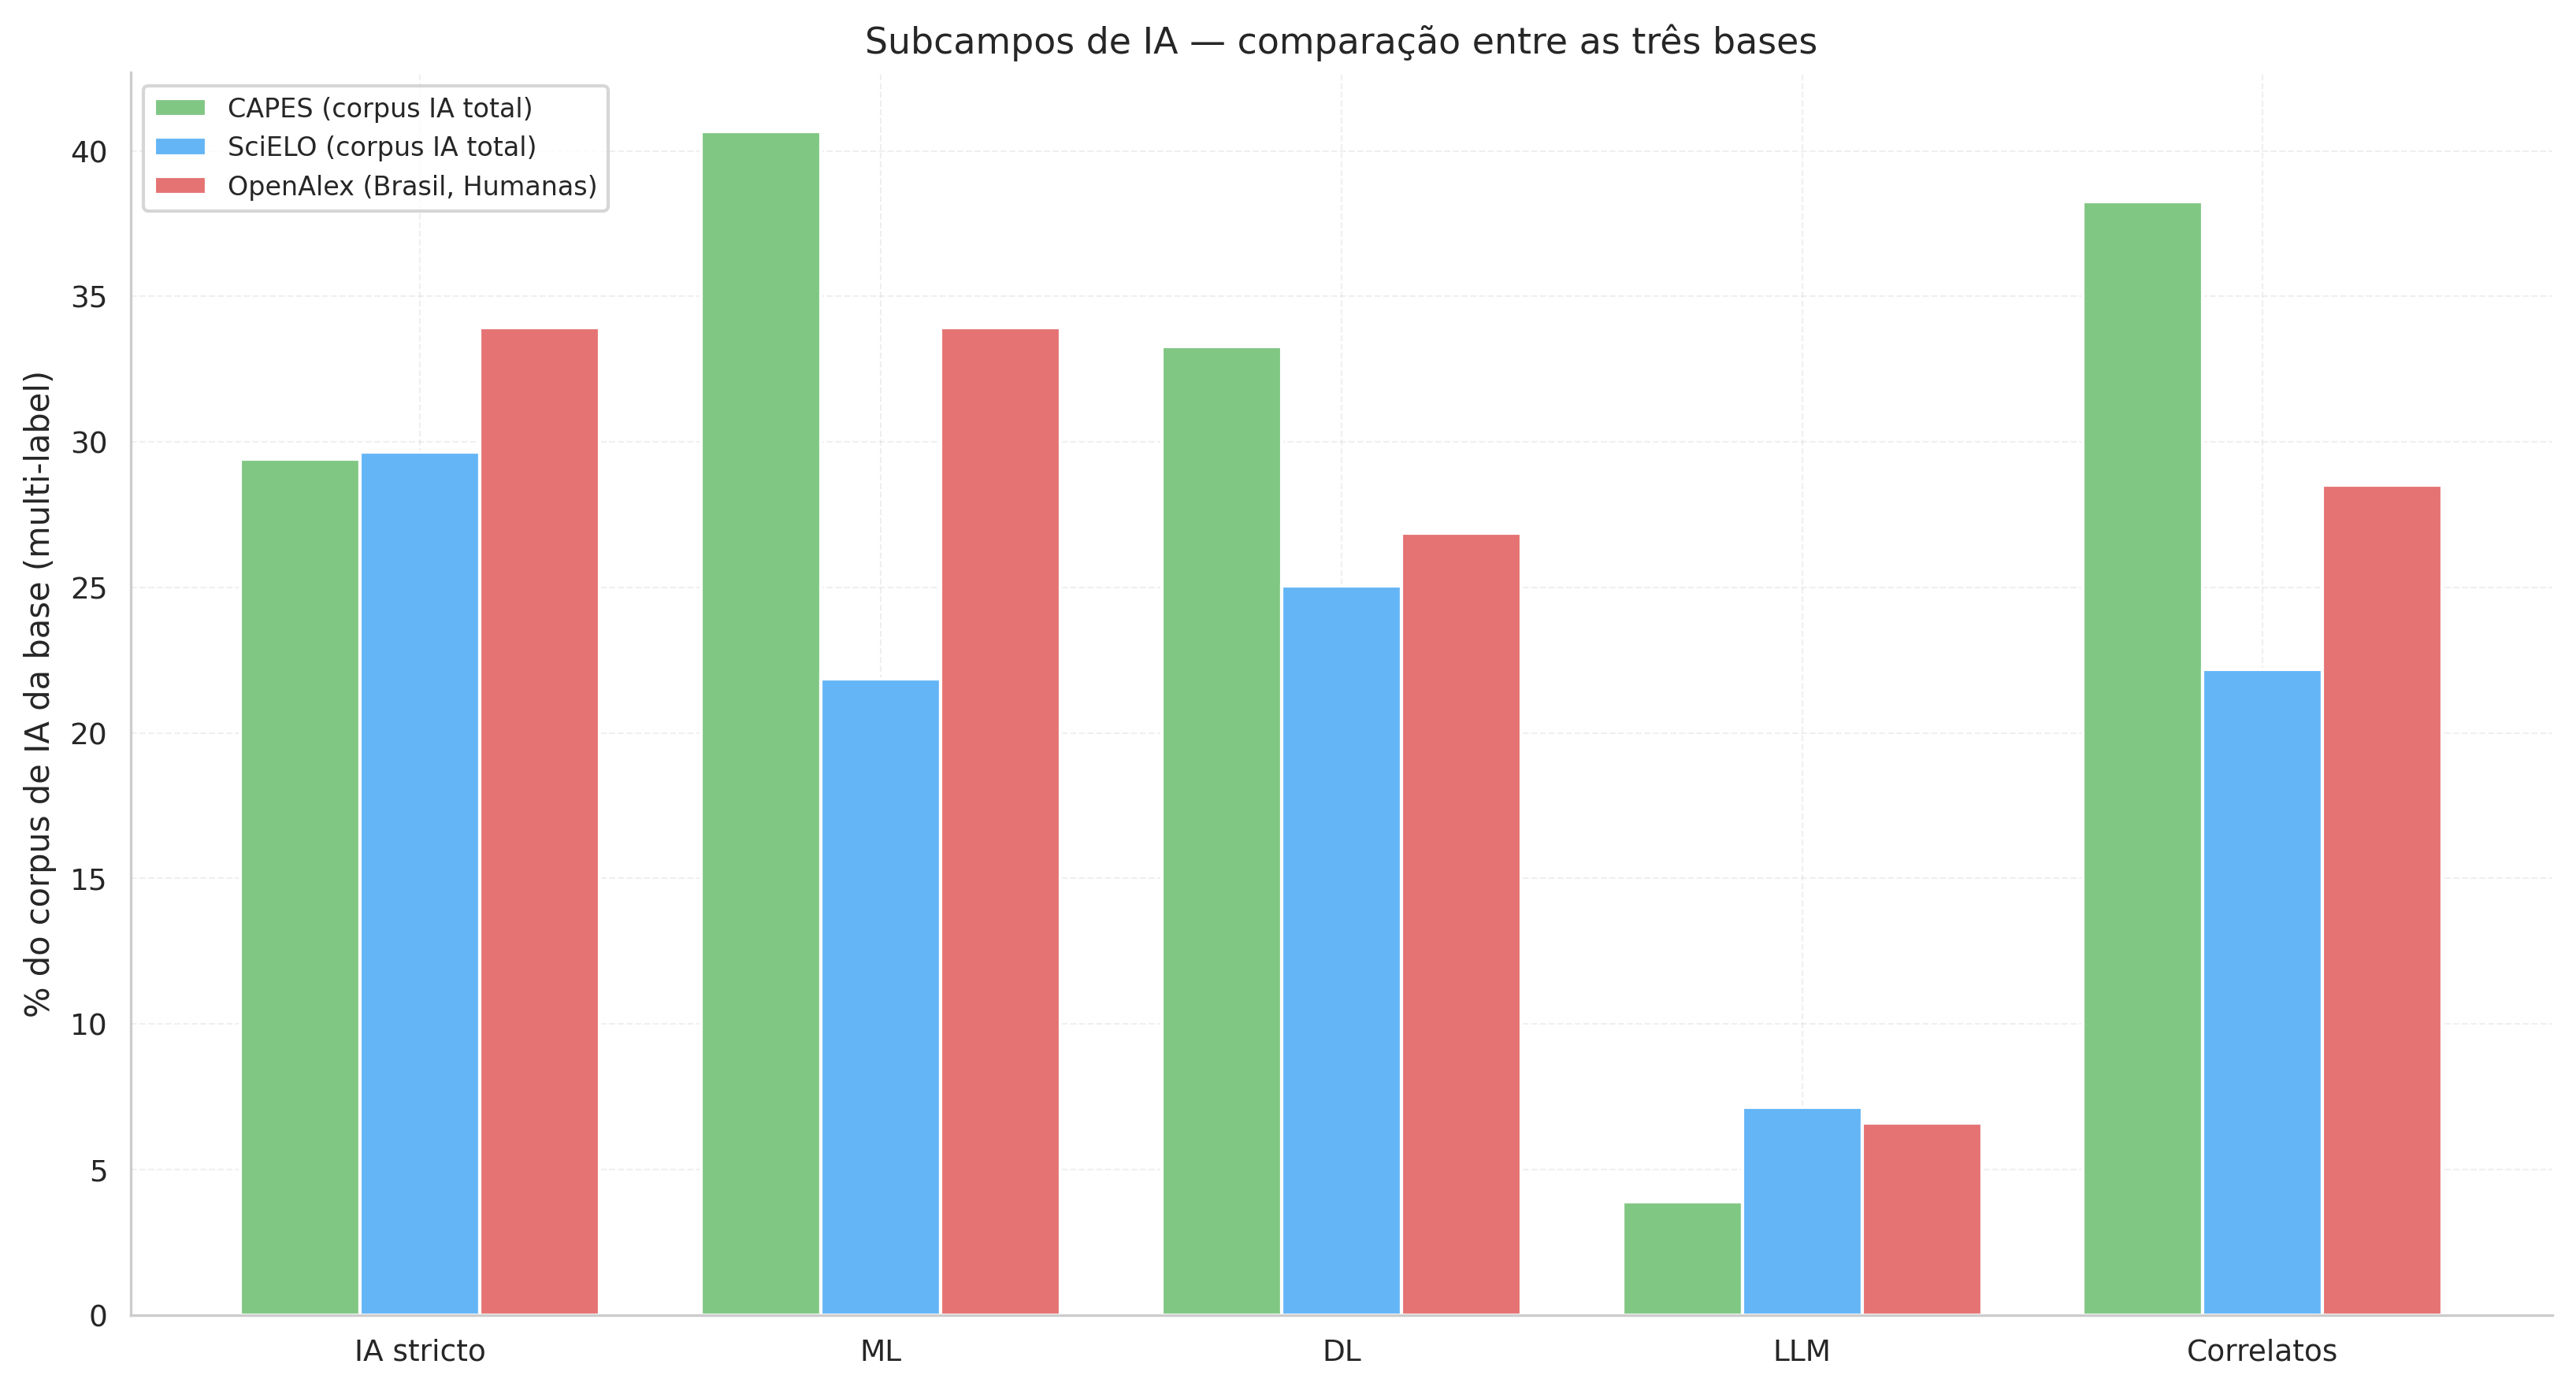
\includegraphics[width=0.95\linewidth]{figuras/openalex_04_subcampos_3bases.png}
  \caption{Peso relativo dos subcampos de IA (rótulos múltiplos; a soma excede
  100\%) em cada fonte. CAPES e SciELO referem-se ao corpus de IA total da base;
  OpenAlex, ao recorte de Humanidades do Brasil (régua de palavra-chave). A
  hierarquia entre IA estrita e aprendizado de máquina (ML) varia entre as
  fontes, e os modelos de linguagem (LLM) constituem o menor subcampo nas três.}
  \label{fig:openalex_04_subcampos_3bases}
  \fonte{Elaboração própria a partir de CAPES, SciELO e OpenAlex.}
\end{figure}

A Figura~\ref{fig:openalex_04_subcampos_3bases} compara o peso dos subcampos ---
IA em sentido estrito, aprendizado de máquina (ML), aprendizado profundo (DL),
modelos de linguagem e IA generativa (LLM) e tecnologias correlatas --- entre as
três fontes. A comparação deve respeitar uma ressalva de escopo: os percentuais
da CAPES e do SciELO referem-se ao corpus de IA \emph{total} de cada base, ao
passo que os do OpenAlex referem-se ao recorte de Humanidades do Brasil. Ainda
assim, dois padrões se destacam. Primeiro, a hierarquia entre IA estrita e ML
varia conforme a fonte: na CAPES o ML predomina (40,7\% contra 29,4\% de IA
estrita), no SciELO a relação se inverte (29,6\% contra 21,9\%), e no OpenAlex os
dois subcampos \emph{empatam} (33,9\% cada). Segundo, os modelos de linguagem e a
IA generativa (LLM) constituem, sistematicamente, o menor subcampo nas três bases
(3,9\% na CAPES, 7,1\% no SciELO e 6,6\% no OpenAlex) --- indício de que, no
período analisado, a virada generativa ainda não se traduzira em produção
acadêmica expressiva nas Humanidades.

% ---------------------------------------------------------------------
\paragraph{Síntese e limitações.} Tomadas em conjunto, as evidências do OpenAlex
internacionalizam o argumento central desta tese: a marginalidade da IA nas
Humanidades brasileiras não decorre de escassez de produção humanística ---
afinal, o país é o segundo maior produtor mundial do conjunto analisado ---, mas
da reduzida permeabilidade desse vasto campo às tecnologias de IA, a menor entre
os grandes produtores. Três limitações devem acompanhar a leitura destes
resultados. \textit{(i)} O OpenAlex privilegia metadados em inglês, o que tende a
subestimar a produção em português (e em chinês), afetando justamente Brasil e
China. \textit{(ii)} Na contagem por país, uma obra é atribuída a cada país de
afiliação de seus autores; os números brasileiros por obra única (bloco
metodológico IV) corrigem essa dupla contagem, mas as comparações internacionais
a mantêm. \textit{(iii)} O ano de 2024 encontra-se subindexado. Nenhuma dessas
limitações, contudo, compromete o achado de fundo, reiterado por três fontes
independentes.

% =====================================================================
%  VISUALIZAÇÕES COMPLEMENTARES (Figuras 05–09)
%  São leituras alternativas dos mesmos dados — use as que melhor servirem
%  à narrativa; não é necessário inserir todas (algumas são redundantes
%  com as Figuras 01–04).
% =====================================================================

% ---------------------------------------------------------------------
\begin{figure}[htbp]
  \centering
  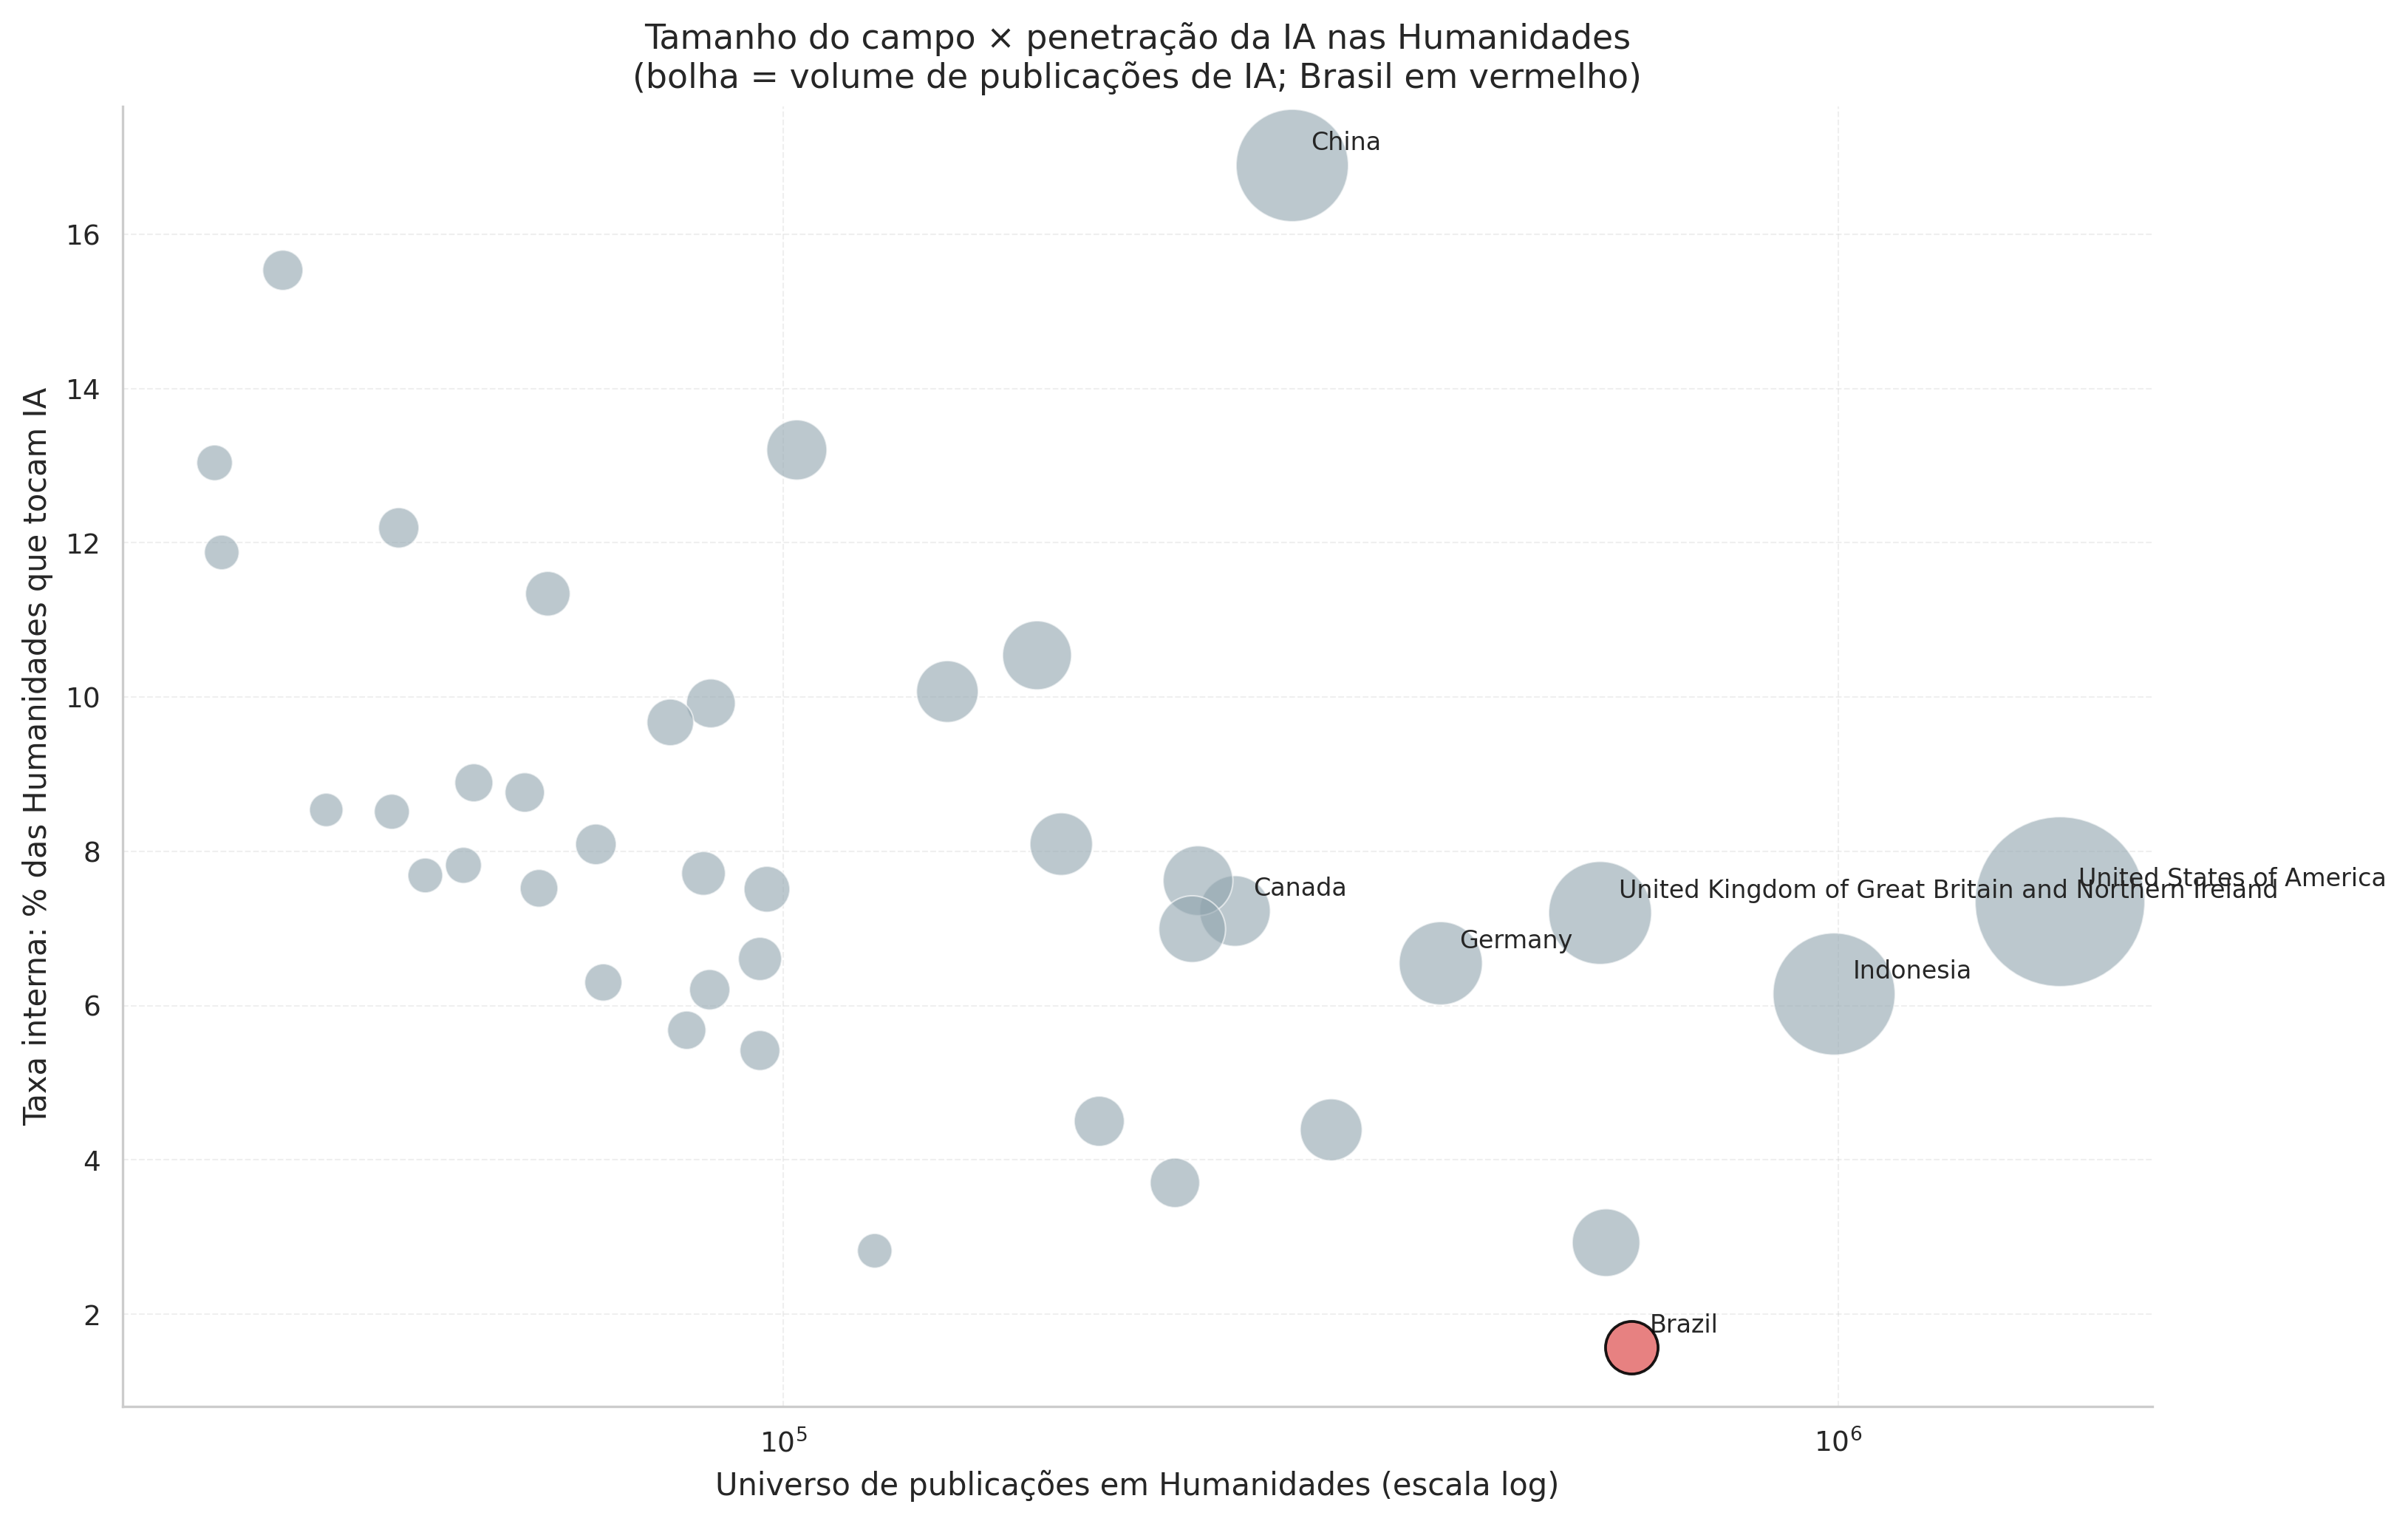
\includegraphics[width=0.95\linewidth]{figuras/openalex_05_bolha_universo_penetracao.png}
  \caption{Dispersão dos quarenta maiores produtores de IA nas Humanidades
  (2016--2024): no eixo horizontal, o tamanho do universo de Humanidades de cada
  país (escala logarítmica); no vertical, a taxa interna de penetração da IA; o
  diâmetro de cada bolha é proporcional ao volume de publicações de IA. O Brasil,
  destacado em vermelho, situa-se entre os maiores universos do mundo, mas no
  patamar inferior de penetração.}
  \label{fig:openalex_05_bolha_universo_penetracao}
  \fonte{Elaboração própria a partir do OpenAlex (2016--2024).}
\end{figure}

A Figura~\ref{fig:openalex_05_bolha_universo_penetracao} cruza, num único plano,
as três dimensões do problema --- tamanho do campo, intensidade da adoção e
volume absoluto de IA. A leitura é imediata: não há associação simples entre
produzir muito em Humanidades e adotar IA. O Brasil aparece como caso
emblemático de \emph{descolamento} entre as duas grandezas --- uma bolha
expressiva, deslocada para a direita (grande universo) e para baixo (baixa
penetração) ---, ao contrário de países como China, Japão ou Países Baixos, que
combinam volume e adoção elevados.

% ---------------------------------------------------------------------
\begin{figure}[htbp]
  \centering
  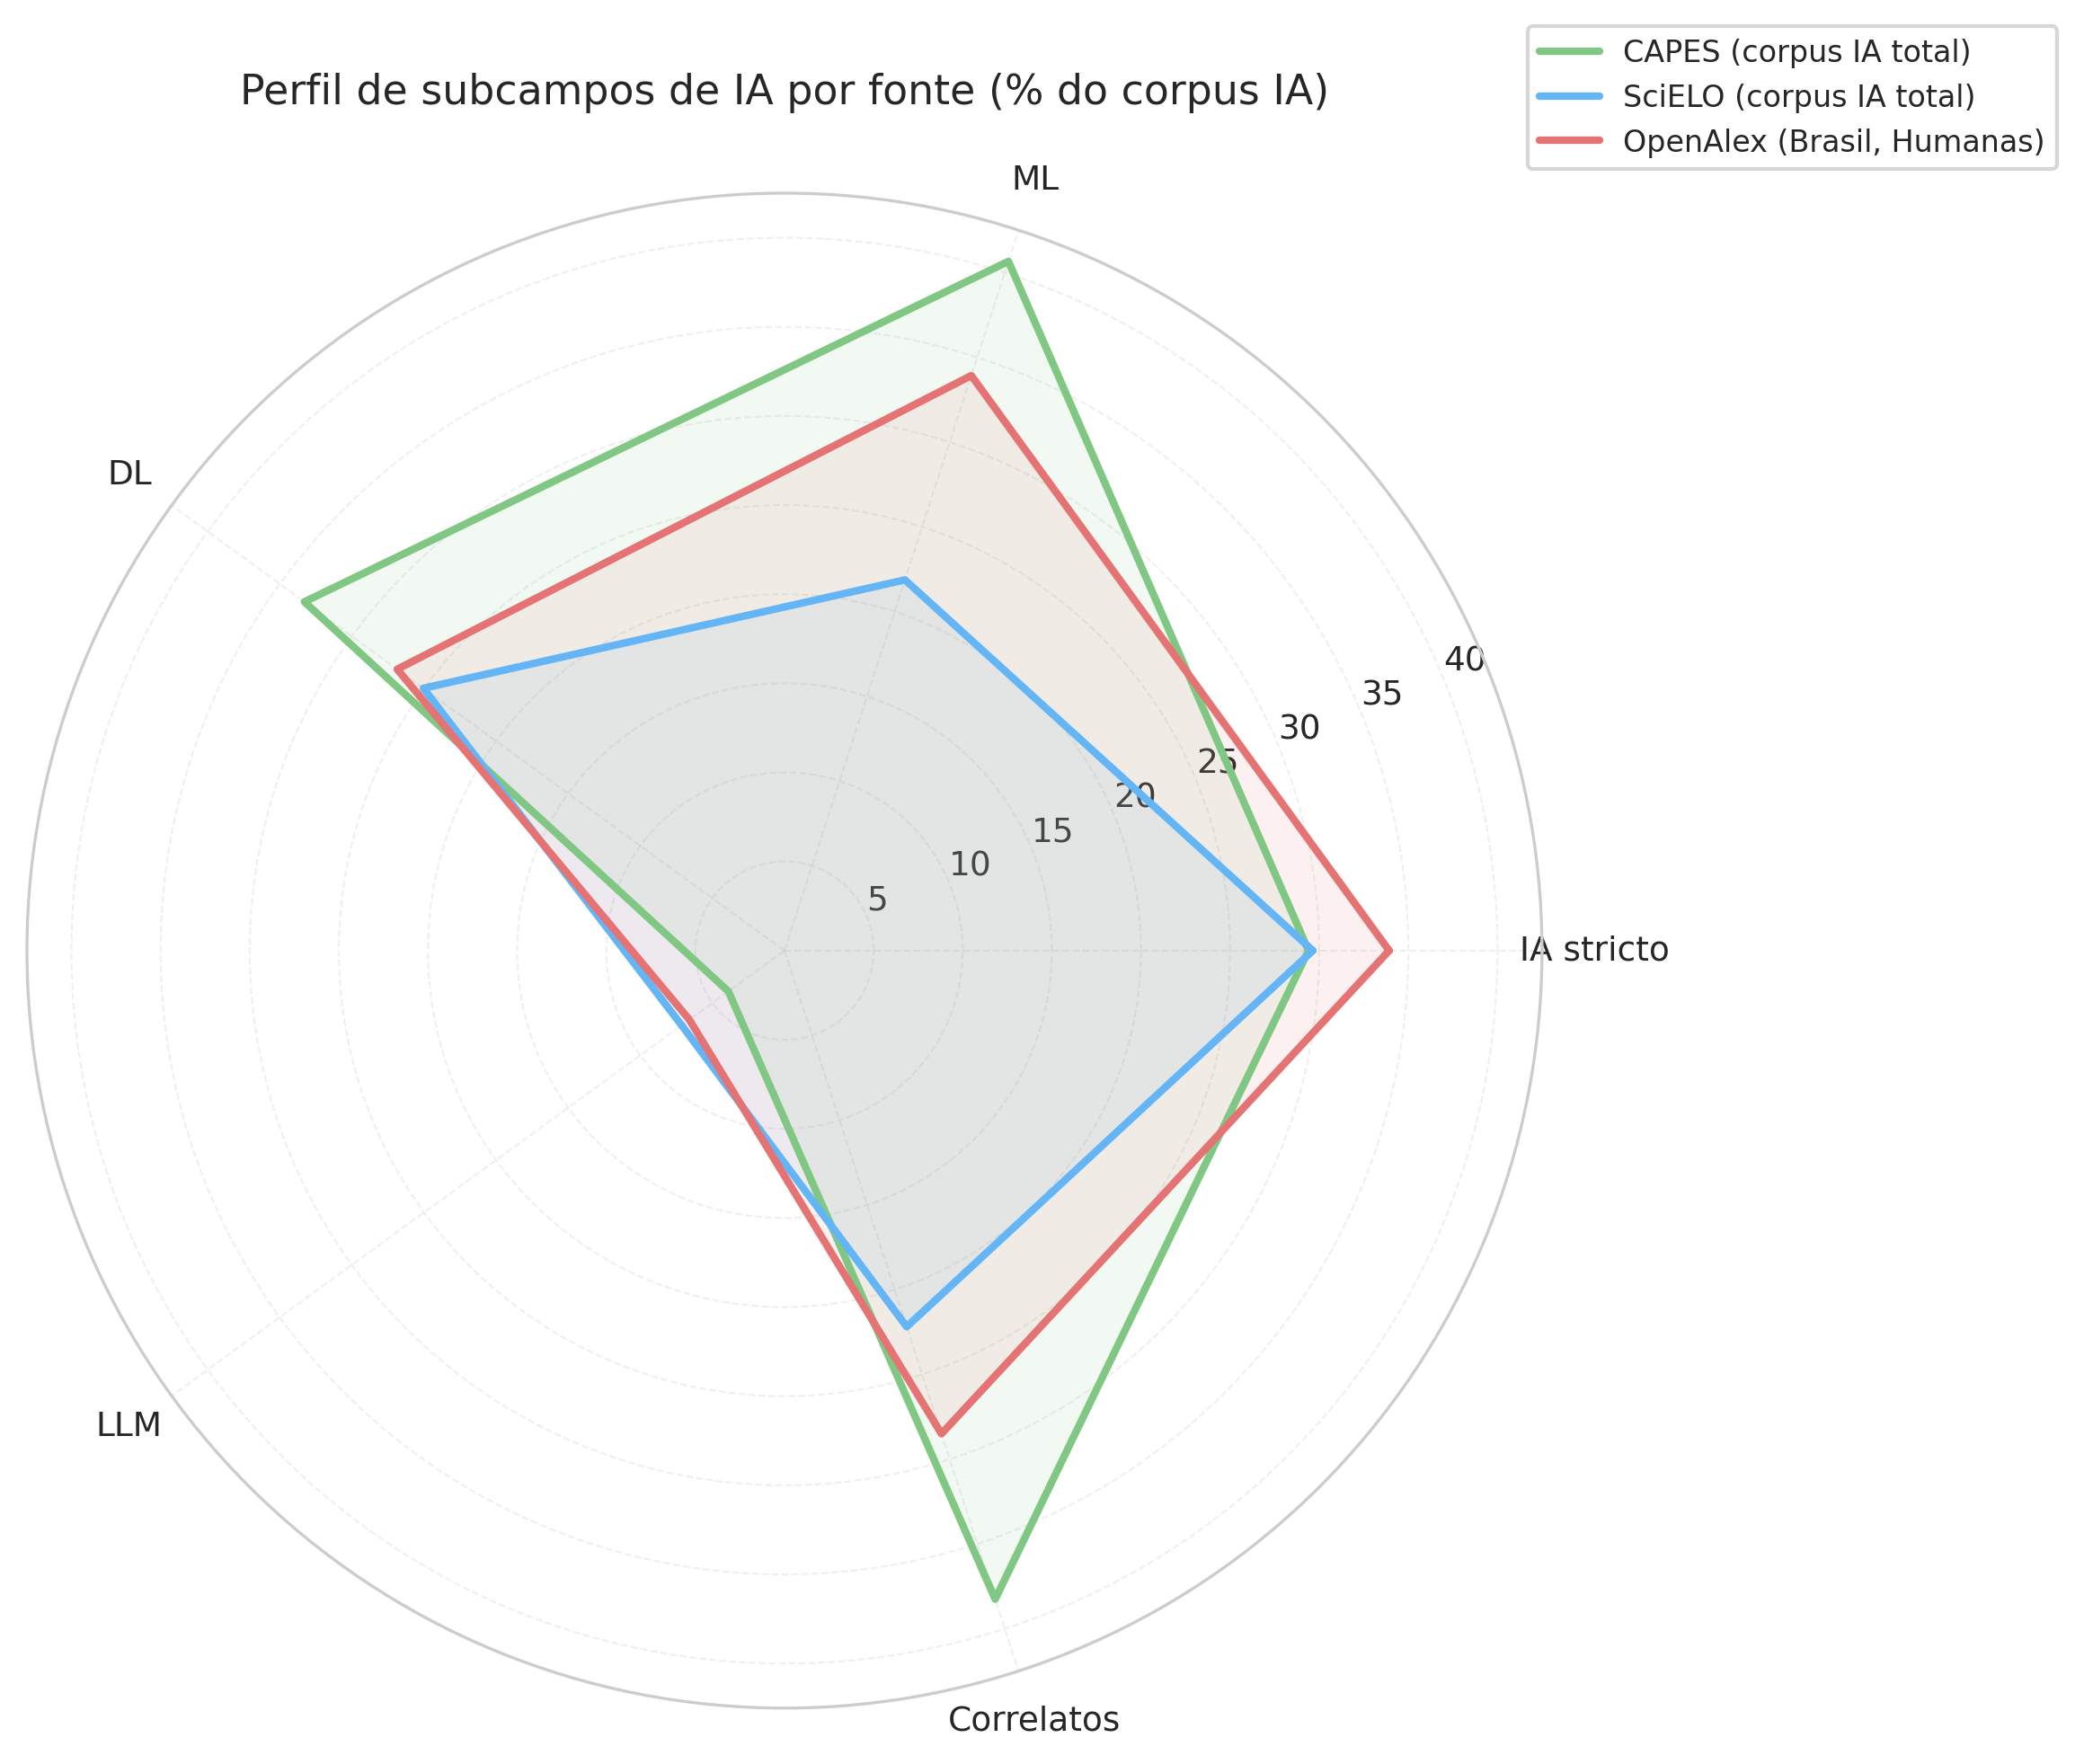
\includegraphics[width=0.8\linewidth]{figuras/openalex_06_radar_subcampos.png}
  \caption{Perfil de subcampos de IA (rótulos múltiplos) em cada fonte,
  representado em diagrama de radar sobre cinco eixos: IA em sentido estrito,
  aprendizado de máquina (ML), aprendizado profundo (DL), modelos de linguagem e
  IA generativa (LLM) e tecnologias correlatas. CAPES e SciELO referem-se ao
  corpus de IA total; OpenAlex, ao recorte de Humanidades do Brasil.}
  \label{fig:openalex_06_radar_subcampos}
  \fonte{Elaboração própria a partir de CAPES, SciELO e OpenAlex.}
\end{figure}

O diagrama de radar da Figura~\ref{fig:openalex_06_radar_subcampos} torna visível
o \emph{formato} de cada perfil disciplinar. O polígono da CAPES estende-se na
direção do ML; o do SciELO, na da IA estrita; o do OpenAlex distribui-se de modo
mais equilibrado entre IA estrita e ML. Em todas as fontes, o eixo dos modelos de
linguagem (LLM) permanece retraído, evidência convergente de que a IA generativa
ainda não reconfigurara a produção das Humanidades no período.

% ---------------------------------------------------------------------
\begin{figure}[htbp]
  \centering
  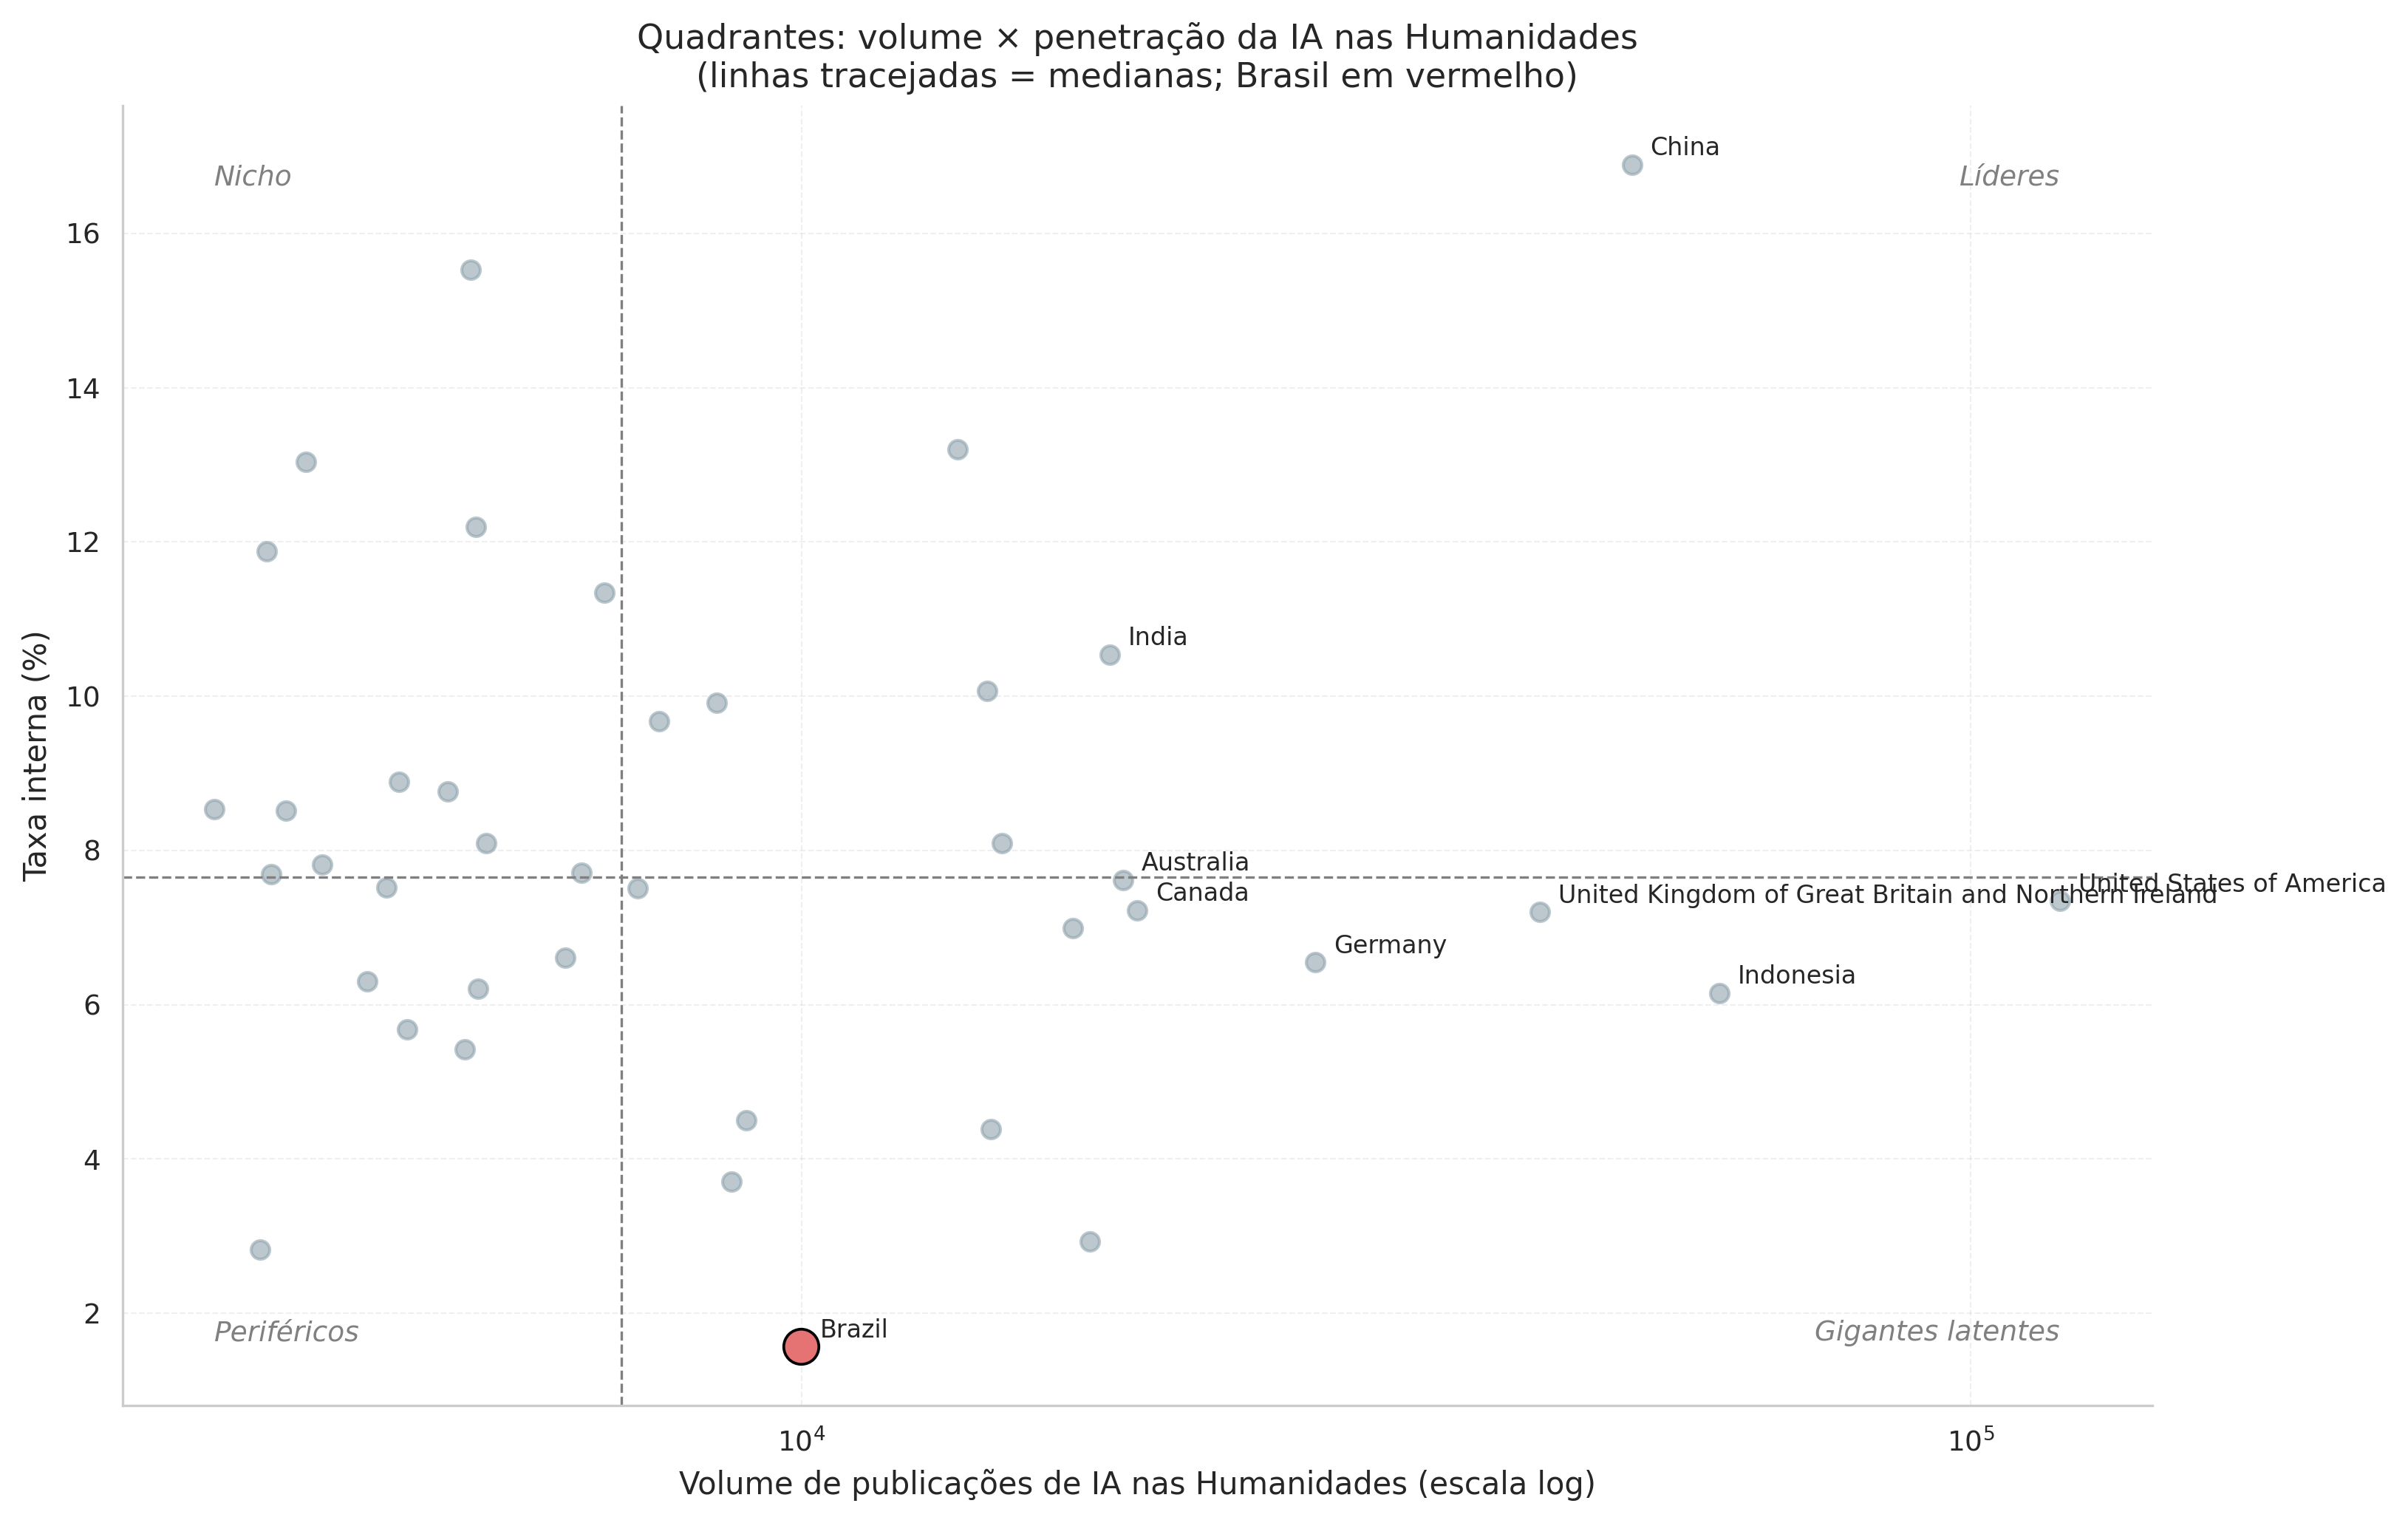
\includegraphics[width=0.95\linewidth]{figuras/openalex_07_quadrante_paises.png}
  \caption{Quadrantes definidos pelas medianas de volume (eixo horizontal,
  logarítmico) e de taxa interna (eixo vertical) entre os quarenta maiores
  produtores de IA nas Humanidades, 2016--2024. Os quatro quadrantes distinguem
  países líderes, de nicho, ``gigantes latentes'' e periféricos. O Brasil,
  destacado, posiciona-se entre os ``gigantes latentes'': alto volume, baixa
  penetração.}
  \label{fig:openalex_07_quadrante_paises}
  \fonte{Elaboração própria a partir do OpenAlex (2016--2024).}
\end{figure}

A tipologia da Figura~\ref{fig:openalex_07_quadrante_paises} nomeia o lugar do
Brasil no cenário internacional. Acima da mediana em volume, mas abaixo dela em
penetração, o país integra o quadrante dos \emph{gigantes latentes} --- grandes
produtores de Humanidades cuja conexão com a IA permanece incipiente. A categoria
sintetiza, numa imagem, o argumento que as três fontes sustentam: há massa
crítica de produção, mas não difusão da IA pelo campo.

% ---------------------------------------------------------------------
\begin{figure}[htbp]
  \centering
  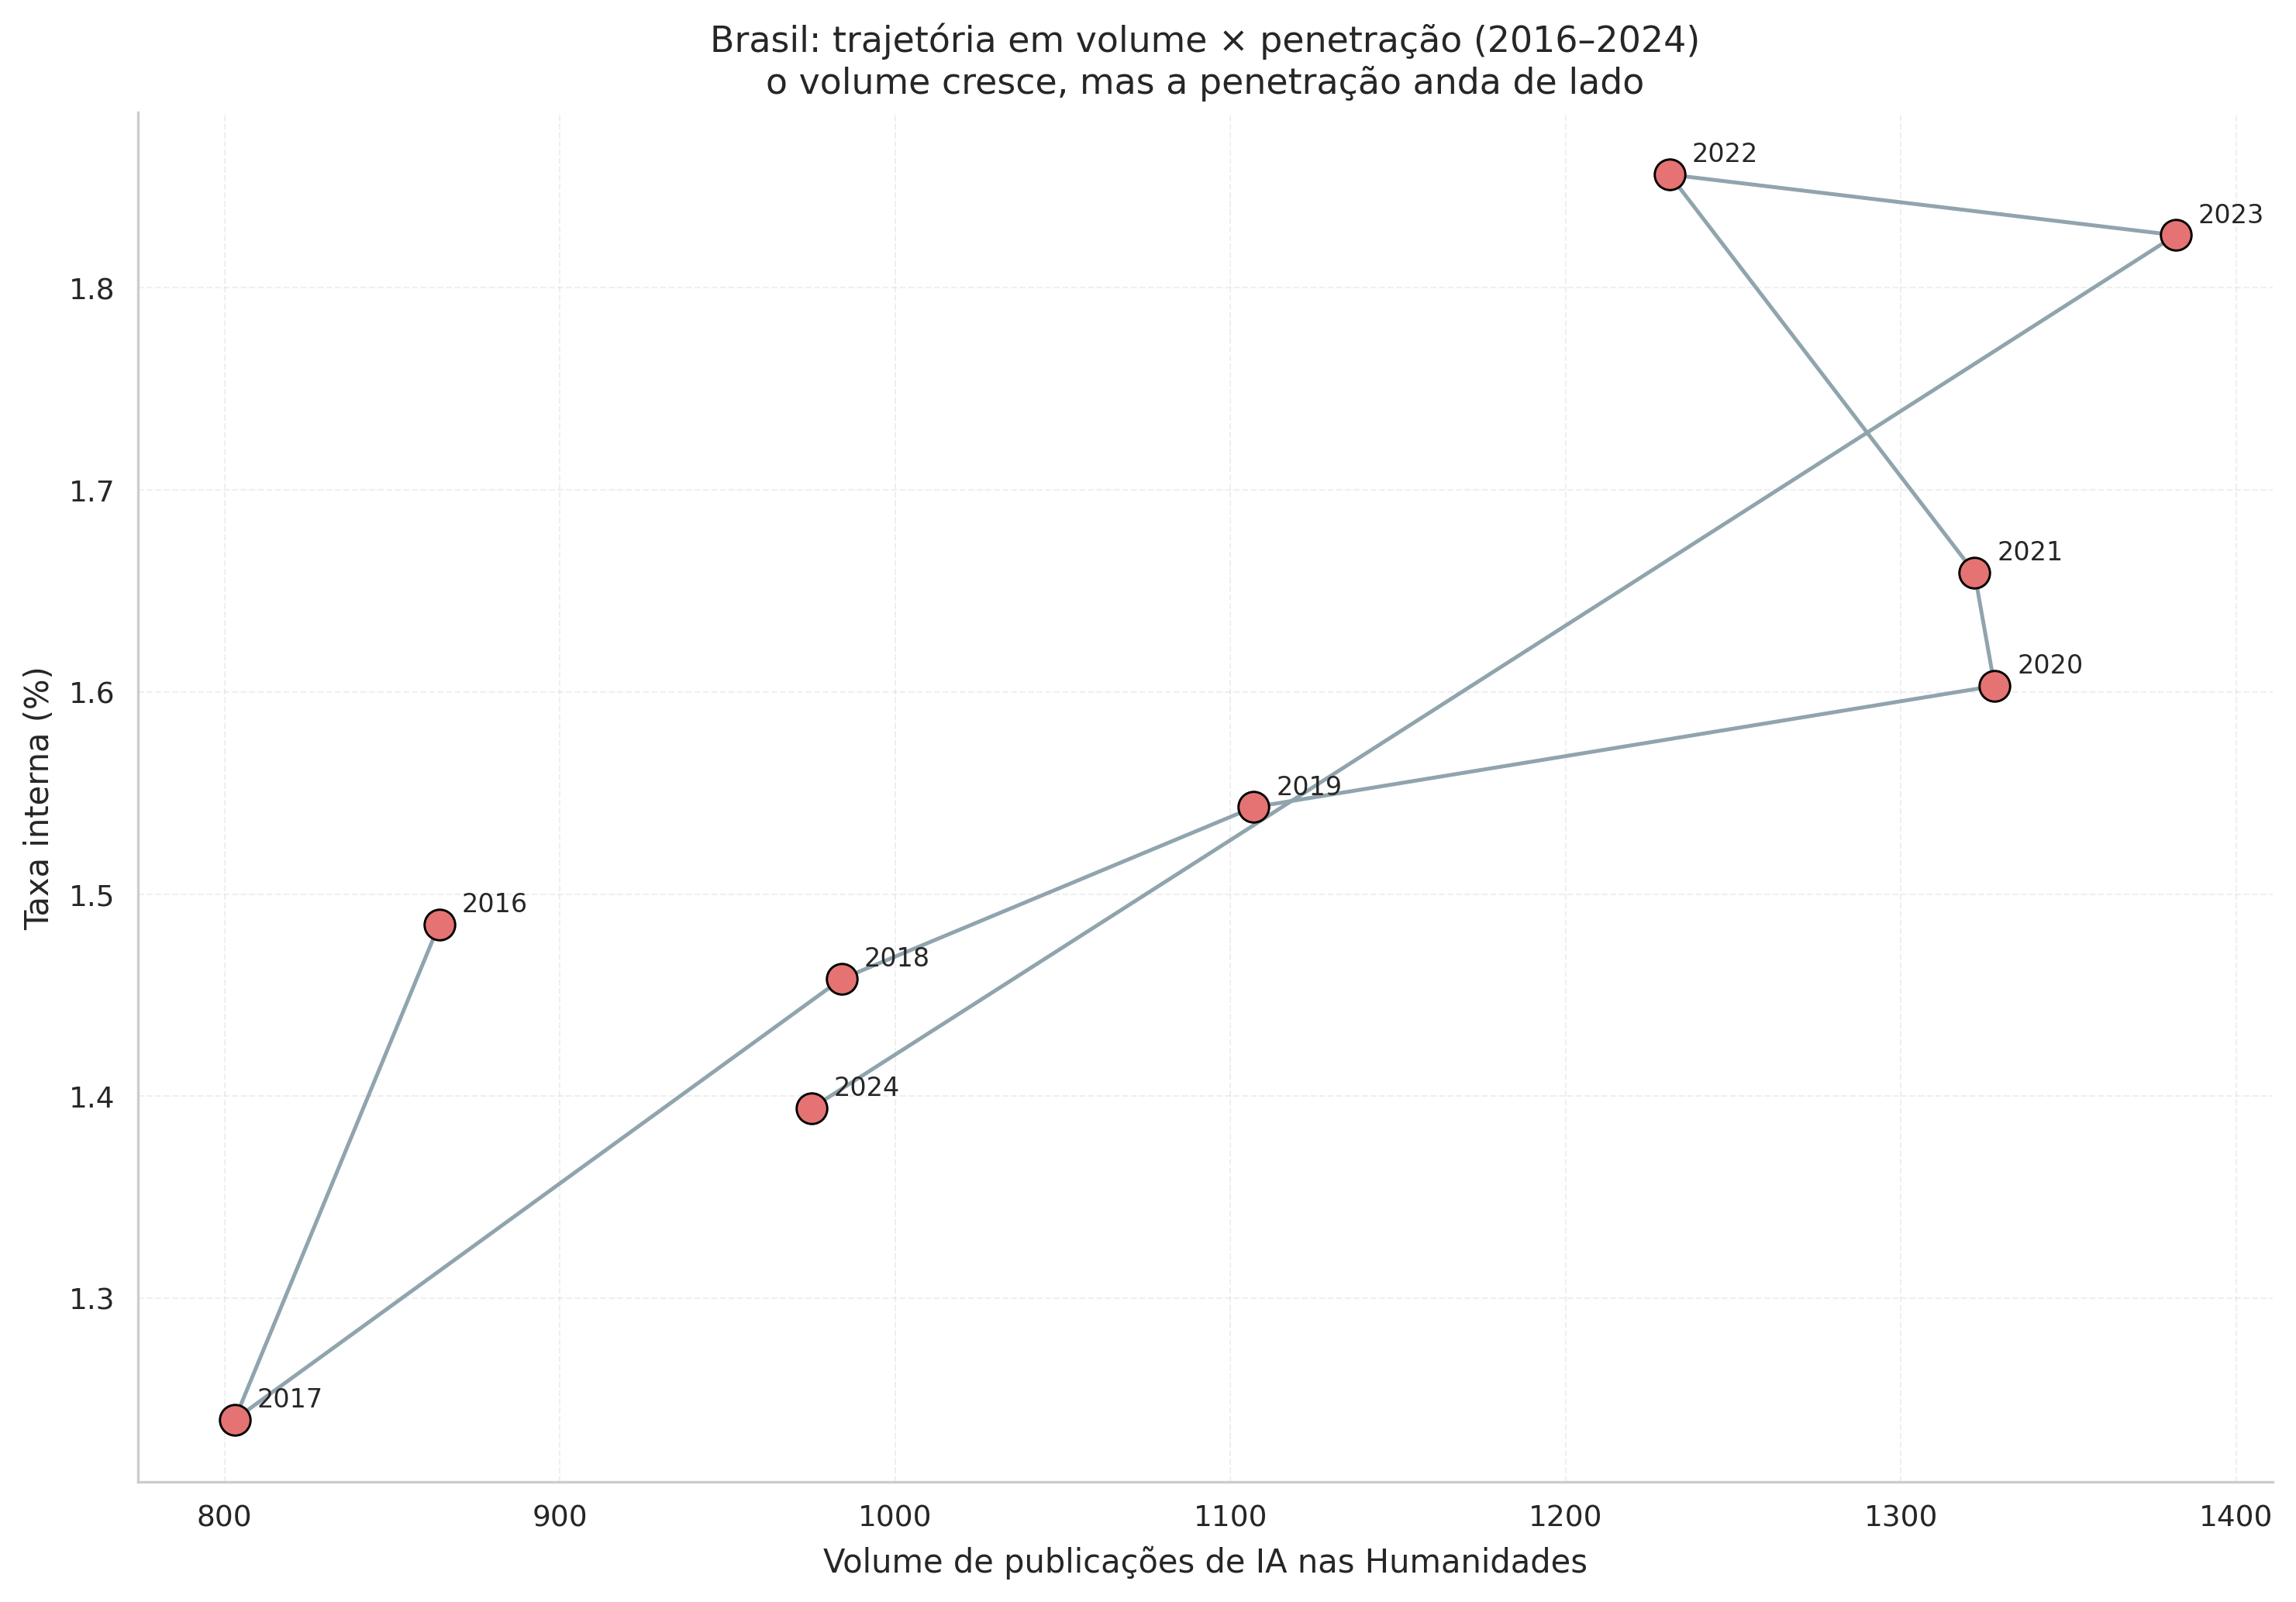
\includegraphics[width=0.85\linewidth]{figuras/openalex_08_trajetoria_brasil.png}
  \caption{Trajetória do Brasil no plano volume × taxa interna, ano a ano, de
  2016 a 2024. Cada ponto é um ano; a linha conecta a sequência temporal. O
  deslocamento predominantemente horizontal indica crescimento do volume sem
  ganho proporcional de penetração.}
  \label{fig:openalex_08_trajetoria_brasil}
  \fonte{Elaboração própria a partir do OpenAlex (2016--2024).}
\end{figure}

A dispersão conectada da Figura~\ref{fig:openalex_08_trajetoria_brasil} acompanha
a evolução brasileira como uma trajetória: os anos avançam sobretudo na
horizontal --- isto é, em volume ---, mas oscilam estreitamente na vertical, sem
romper o teto de cerca de 1,9\% de penetração. O Brasil, em suma, produz a cada
ano mais trabalhos de IA nas Humanidades, sem que isso represente uma abertura
proporcional do campo à temática.

% ---------------------------------------------------------------------
\begin{figure}[htbp]
  \centering
  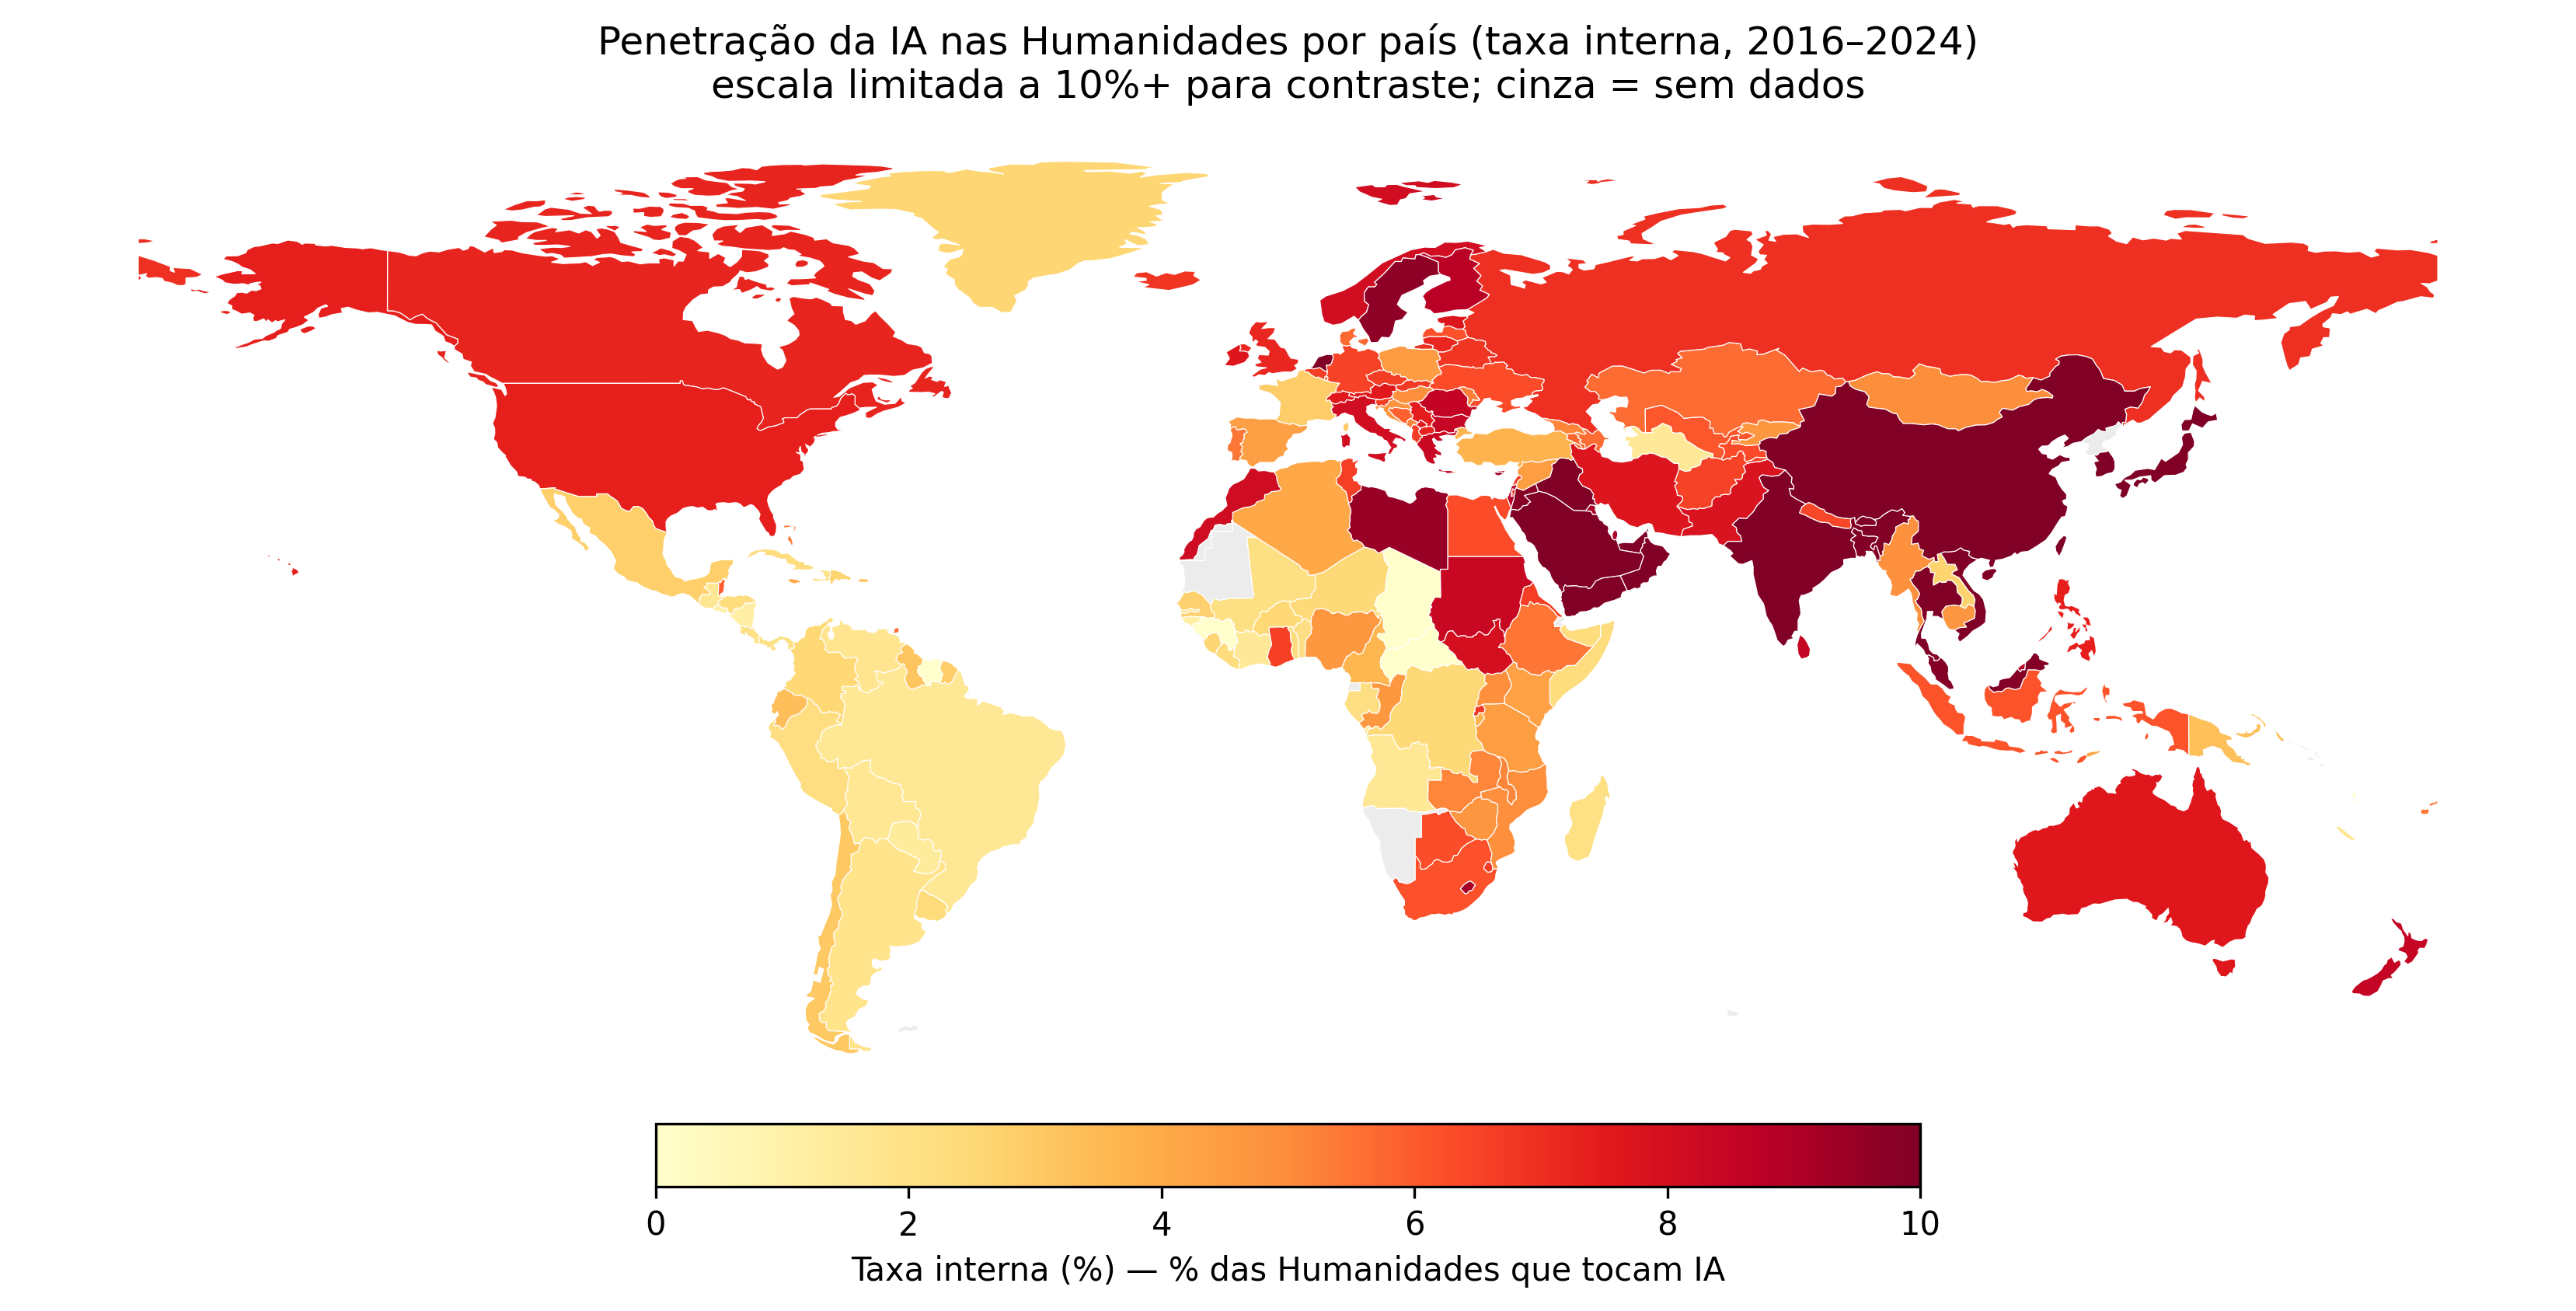
\includegraphics[width=0.95\linewidth]{figuras/openalex_09_mapa_taxa_interna.png}
  \caption{Mapa-múndi coroplético da taxa interna de penetração da IA nas
  Humanidades (2016--2024), para 167 países. Tons mais escuros indicam maior
  fração das Humanidades nacionais dedicada à IA; a escala de cor é limitada a
  10\%+ para preservar contraste (a China atinge 16,9\%); países em cinza não têm
  dados na fonte.}
  \label{fig:openalex_09_mapa_taxa_interna}
  \fonte{Elaboração própria a partir do OpenAlex (2016--2024).}
\end{figure}

Por fim, o mapa da Figura~\ref{fig:openalex_09_mapa_taxa_interna} distribui
geograficamente a penetração da IA nas Humanidades. Além de situar o Brasil em
relação aos demais países de um só relance, a representação revela que a adoção
intensa não se concentra numa única região do globo, mas aparece em contextos
diversos --- da Ásia Oriental ao norte da Europa ---, reforçando que a baixa
permeabilidade observada no Brasil é uma característica do caso nacional, e não
um padrão geral do hemisfério ou do nível de desenvolvimento.

% =====================================================================
%  COMPOSIÇÃO TEMÁTICA — de que é feita a produção brasileira (Figuras 10–15)
%  Responde "sobre o que o Brasil pesquisa em Humanidades?".
%  Obs.: a Figura 12 (painel) é a versão combinada das Figuras 13–15
%  (desmembradas); use uma OU outra, conforme o espaço da tese.
% =====================================================================

\subsection{De que é feita a produção brasileira em Ciências Humanas}

Estabelecida a marginalidade da IA, cabe perguntar \emph{sobre o que}, afinal,
o Brasil pesquisa em Humanidades. A Figura~\ref{fig:openalex_10_treemap_temas}
decompõe o universo de 636.607 publicações nas áreas (\textit{subfields}) que o
constituem.

\begin{figure}[htbp]
  \centering
  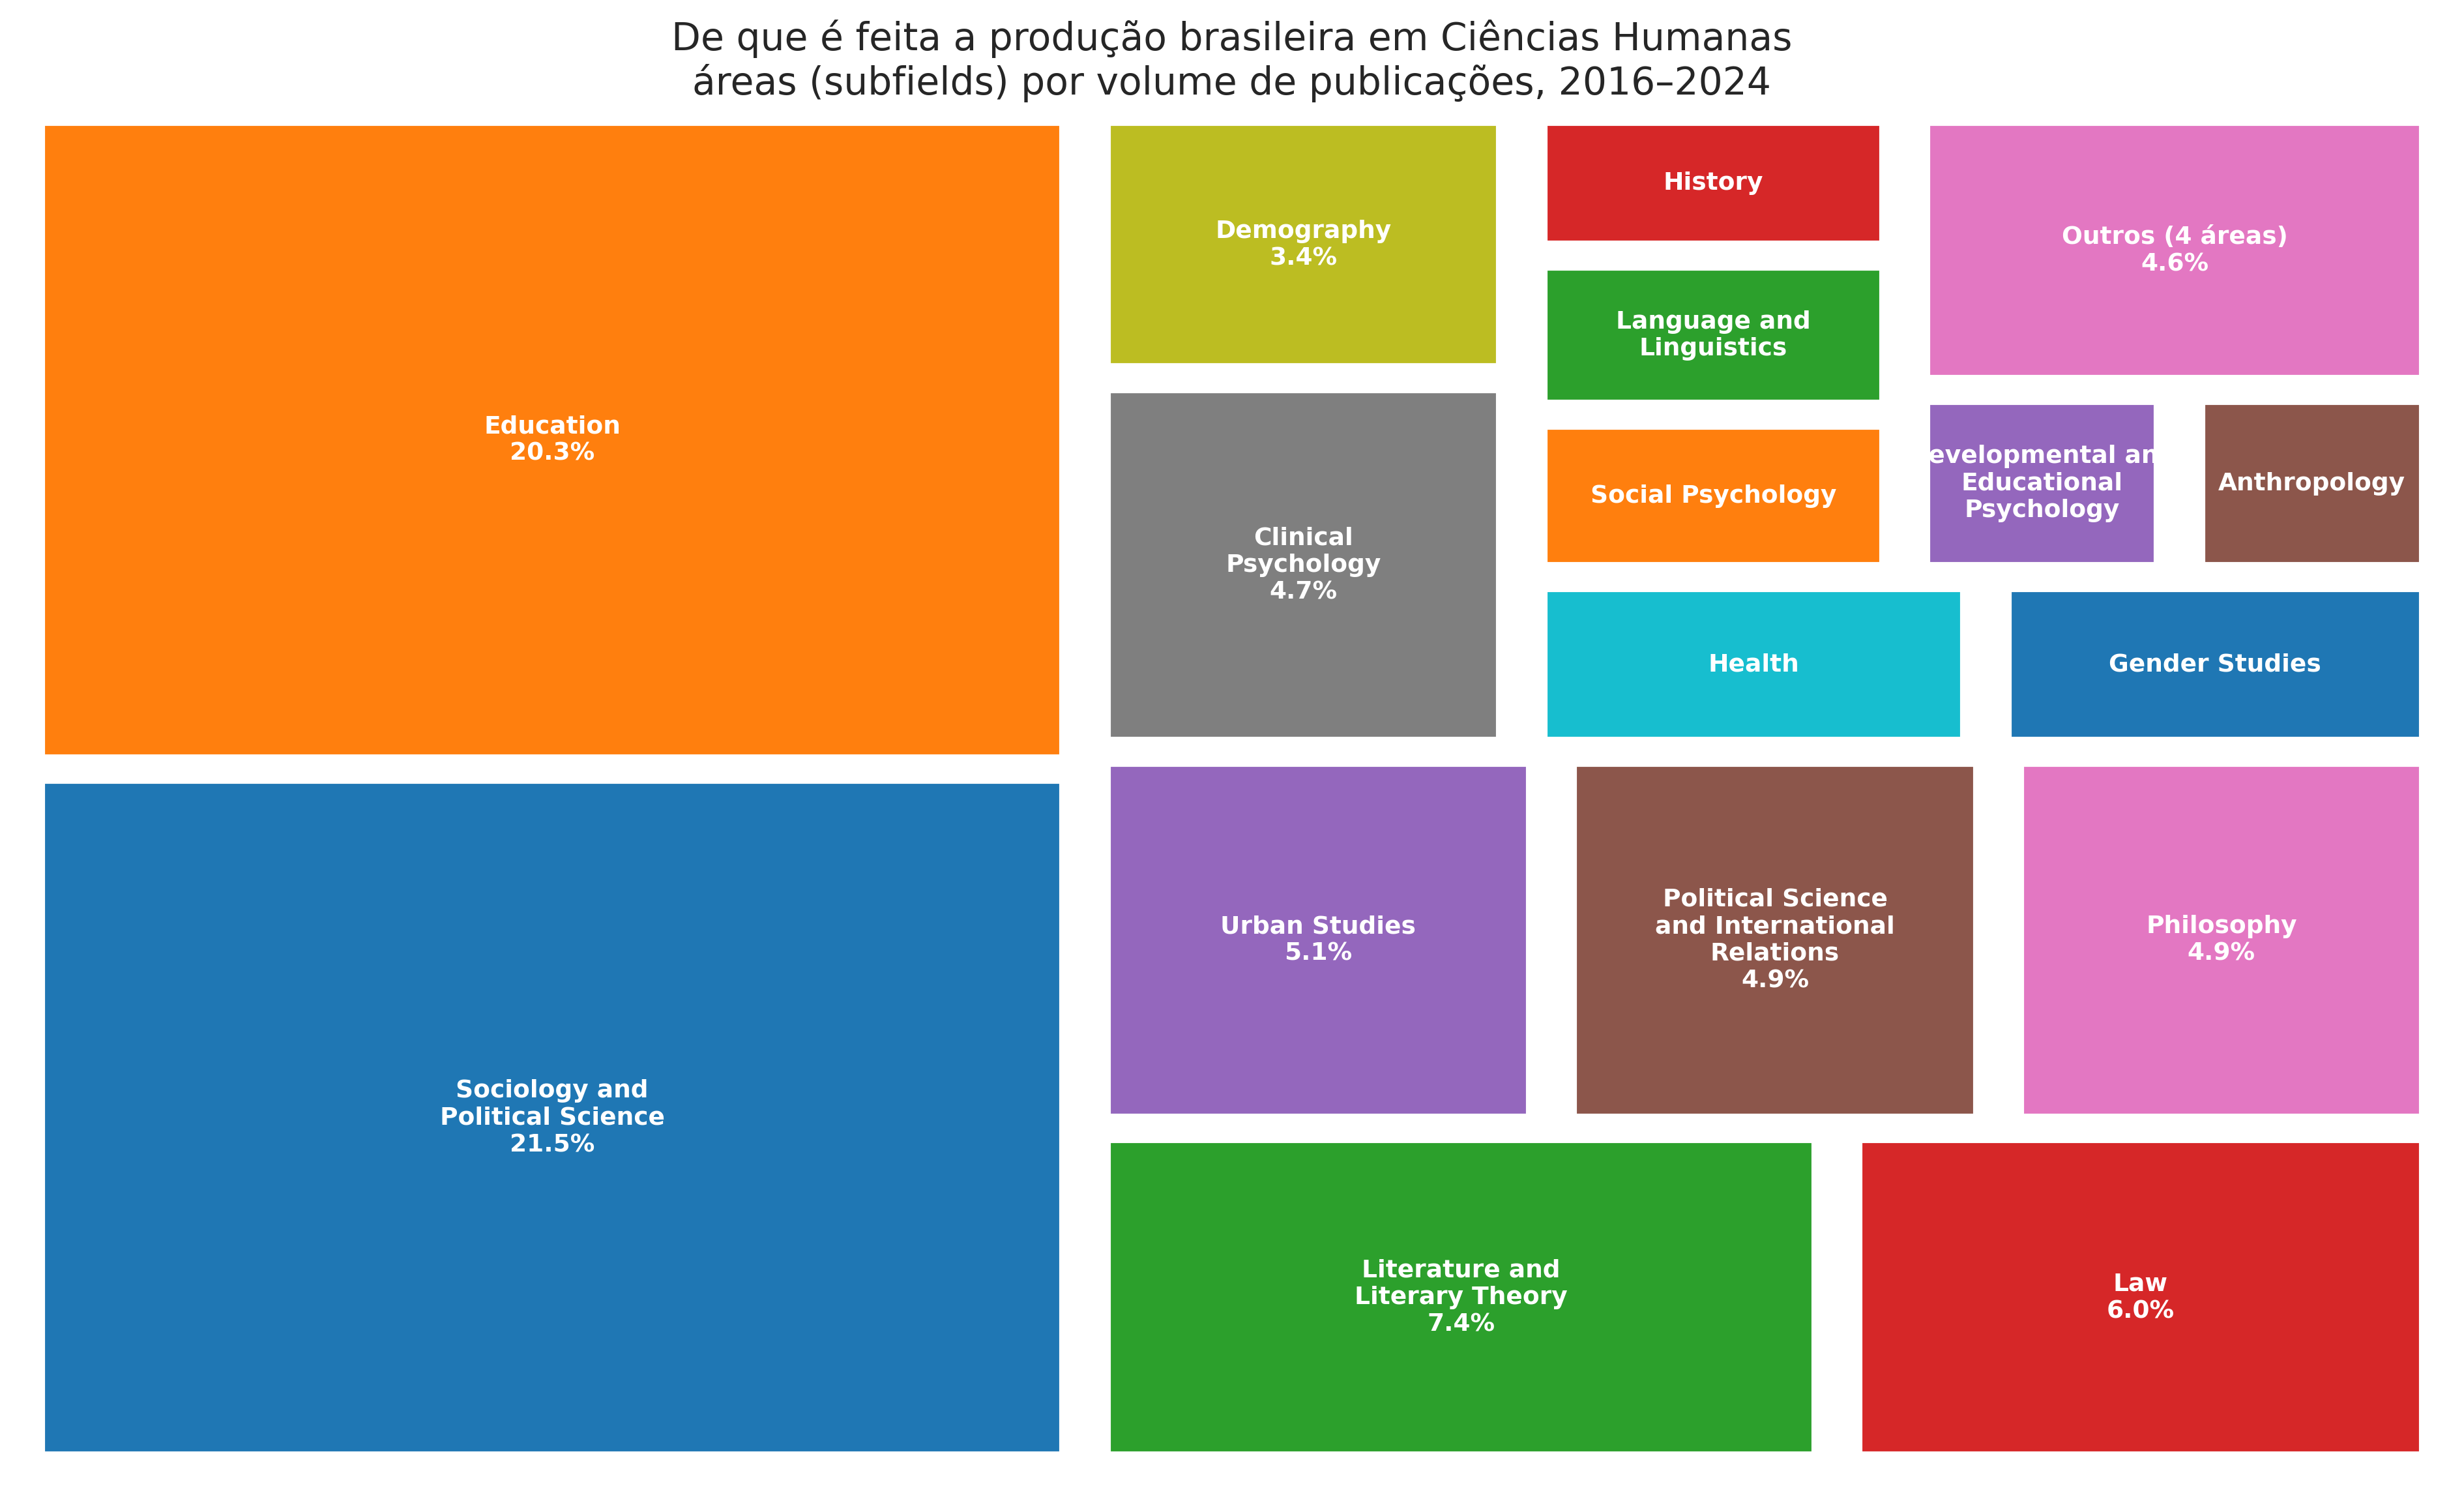
\includegraphics[width=0.95\linewidth]{figuras/openalex_10_treemap_temas.png}
  \caption{Composição da produção brasileira em Ciências Humanas (2016--2024) por
  área (\textit{subfield}), em mapa de árvore: a área de cada retângulo é
  proporcional ao volume de publicações. Mostram-se as dezesseis maiores áreas e
  um bloco agregando as demais.}
  \label{fig:openalex_10_treemap_temas}
  \fonte{Elaboração própria a partir do OpenAlex (2016--2024).}
\end{figure}

Dois blocos dominam a paisagem: \textit{Sociology and Political Science}
(21,5\%) e \textit{Education} (20,3\%) somam, juntos, cerca de 42\% de toda a
produção. A Humanidade brasileira é, portanto, em primeiro lugar, uma ciência da
sociedade e da educação; literatura, direito, estudos urbanos e filosofia compõem
um segundo escalão.

\begin{figure}[htbp]
  \centering
  \includegraphics[width=0.95\linewidth]{figuras/openalex_11_topics_temas.png}
  \caption{Temas específicos (\textit{topics}) mais frequentes no conjunto das
  Ciências Humanas brasileiras (2016--2024). O rótulo ``IA \%'' indica a fração
  de cada tema que toca o campo da inteligência artificial.}
  \label{fig:openalex_11_topics_temas}
  \fonte{Elaboração própria a partir do OpenAlex (2016--2024).}
\end{figure}

Descendo ao nível dos temas específicos (Figura~\ref{fig:openalex_11_topics_temas}),
e em particular ao recorte das ciências sociais
(Figuras~\ref{fig:openalex_13_anthropology}, \ref{fig:openalex_14_sociology}
e~\ref{fig:openalex_15_political_science}), três padrões se confirmam. Primeiro,
a \textbf{centralidade da educação}: ``Education and Digital Technologies'' é o
maior tema dentro da Sociologia e Ciência Política, e ``Education and Public
Policy'' domina a Ciência Política e Relações Internacionais. Segundo, a
\textbf{vocação histórica da Antropologia}, cujo maior tema é, de longe, ``History
of Colonial Brazil'', seguido de colonialismo, história africana e estudos
indígenas. Terceiro, a IA só alcança penetração relevante em \textbf{nichos
digitais} de pequeno volume --- desinformação, redes sociais, governo eletrônico,
``Artificial Intelligence in Law'' ---, ausente dos grandes temas que estruturam
o campo.

\begin{figure}[htbp]
  \centering
  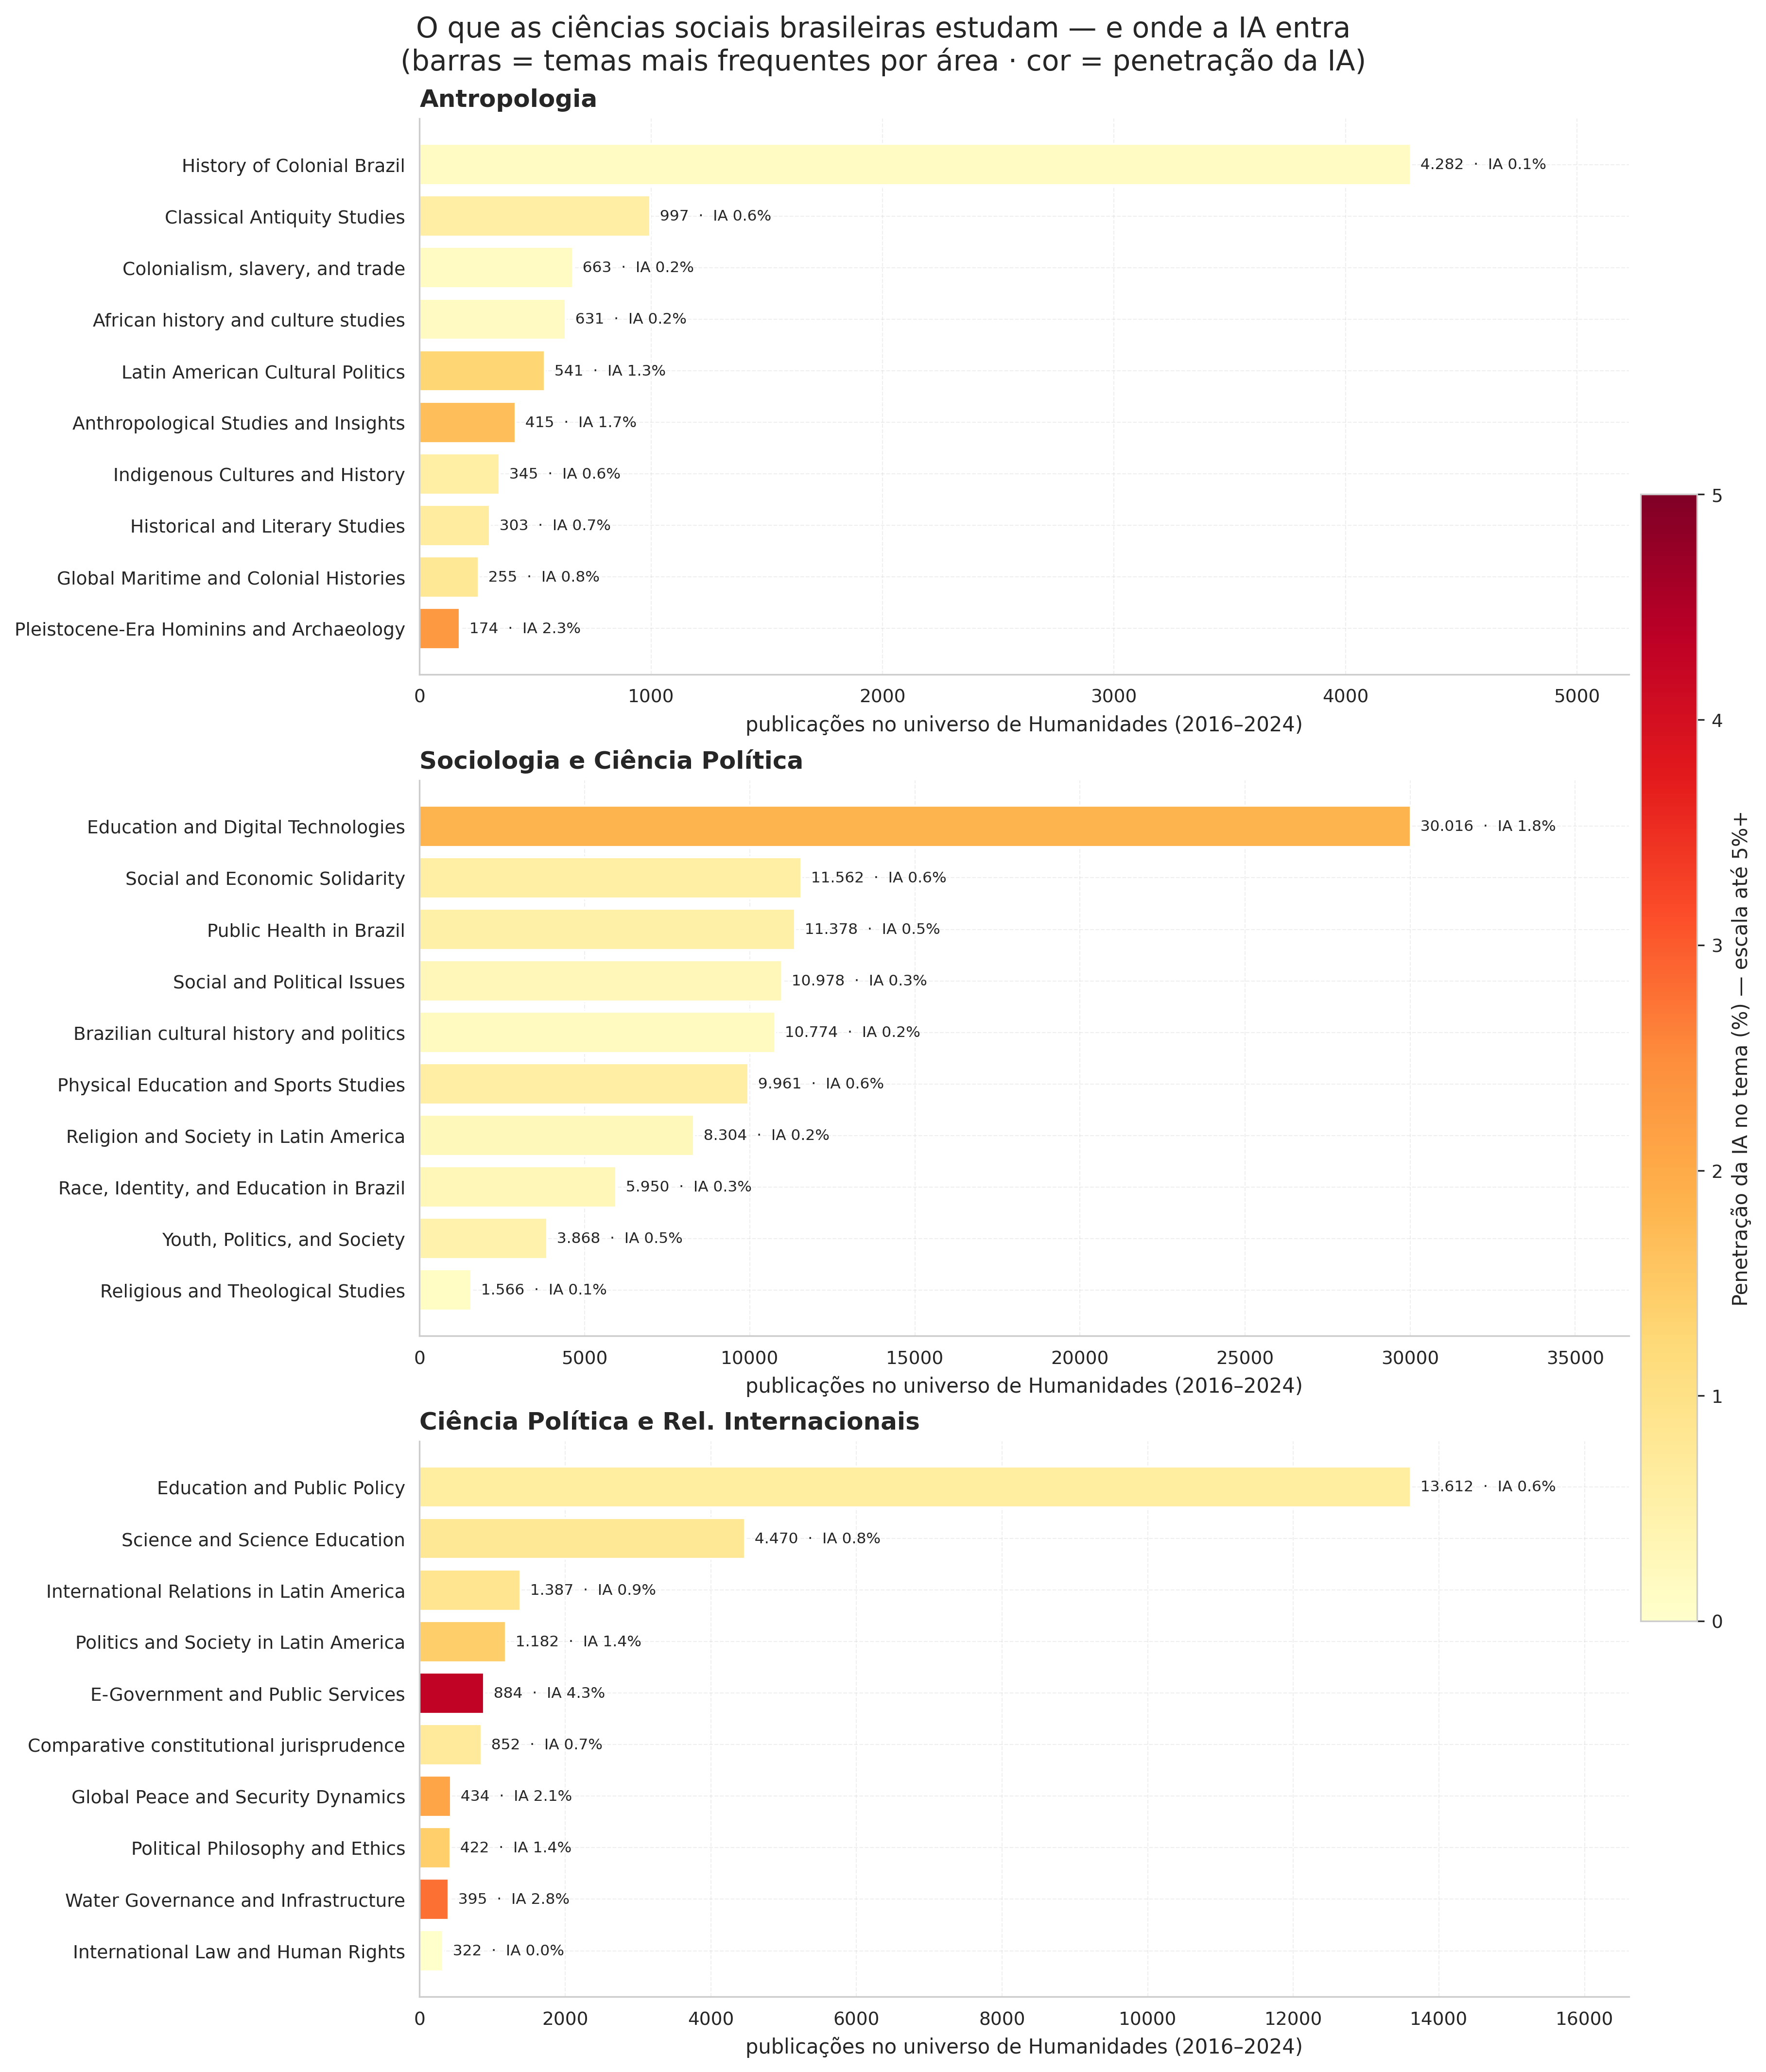
\includegraphics[width=0.95\linewidth]{figuras/openalex_12_painel_ciencias_sociais.png}
  \caption{Temas mais frequentes nas três áreas das ciências sociais brasileiras
  (Antropologia; Sociologia e Ciência Política; Ciência Política e Relações
  Internacionais), 2016--2024, com a penetração da IA por tema indicada no rótulo
  (``IA \%''). Versão em painel das Figuras~\ref{fig:openalex_13_anthropology}
  a~\ref{fig:openalex_15_political_science}.}
  \label{fig:openalex_12_painel_ciencias_sociais}
  \fonte{Elaboração própria a partir do OpenAlex (2016--2024).}
\end{figure}

\begin{figure}[htbp]
  \centering
  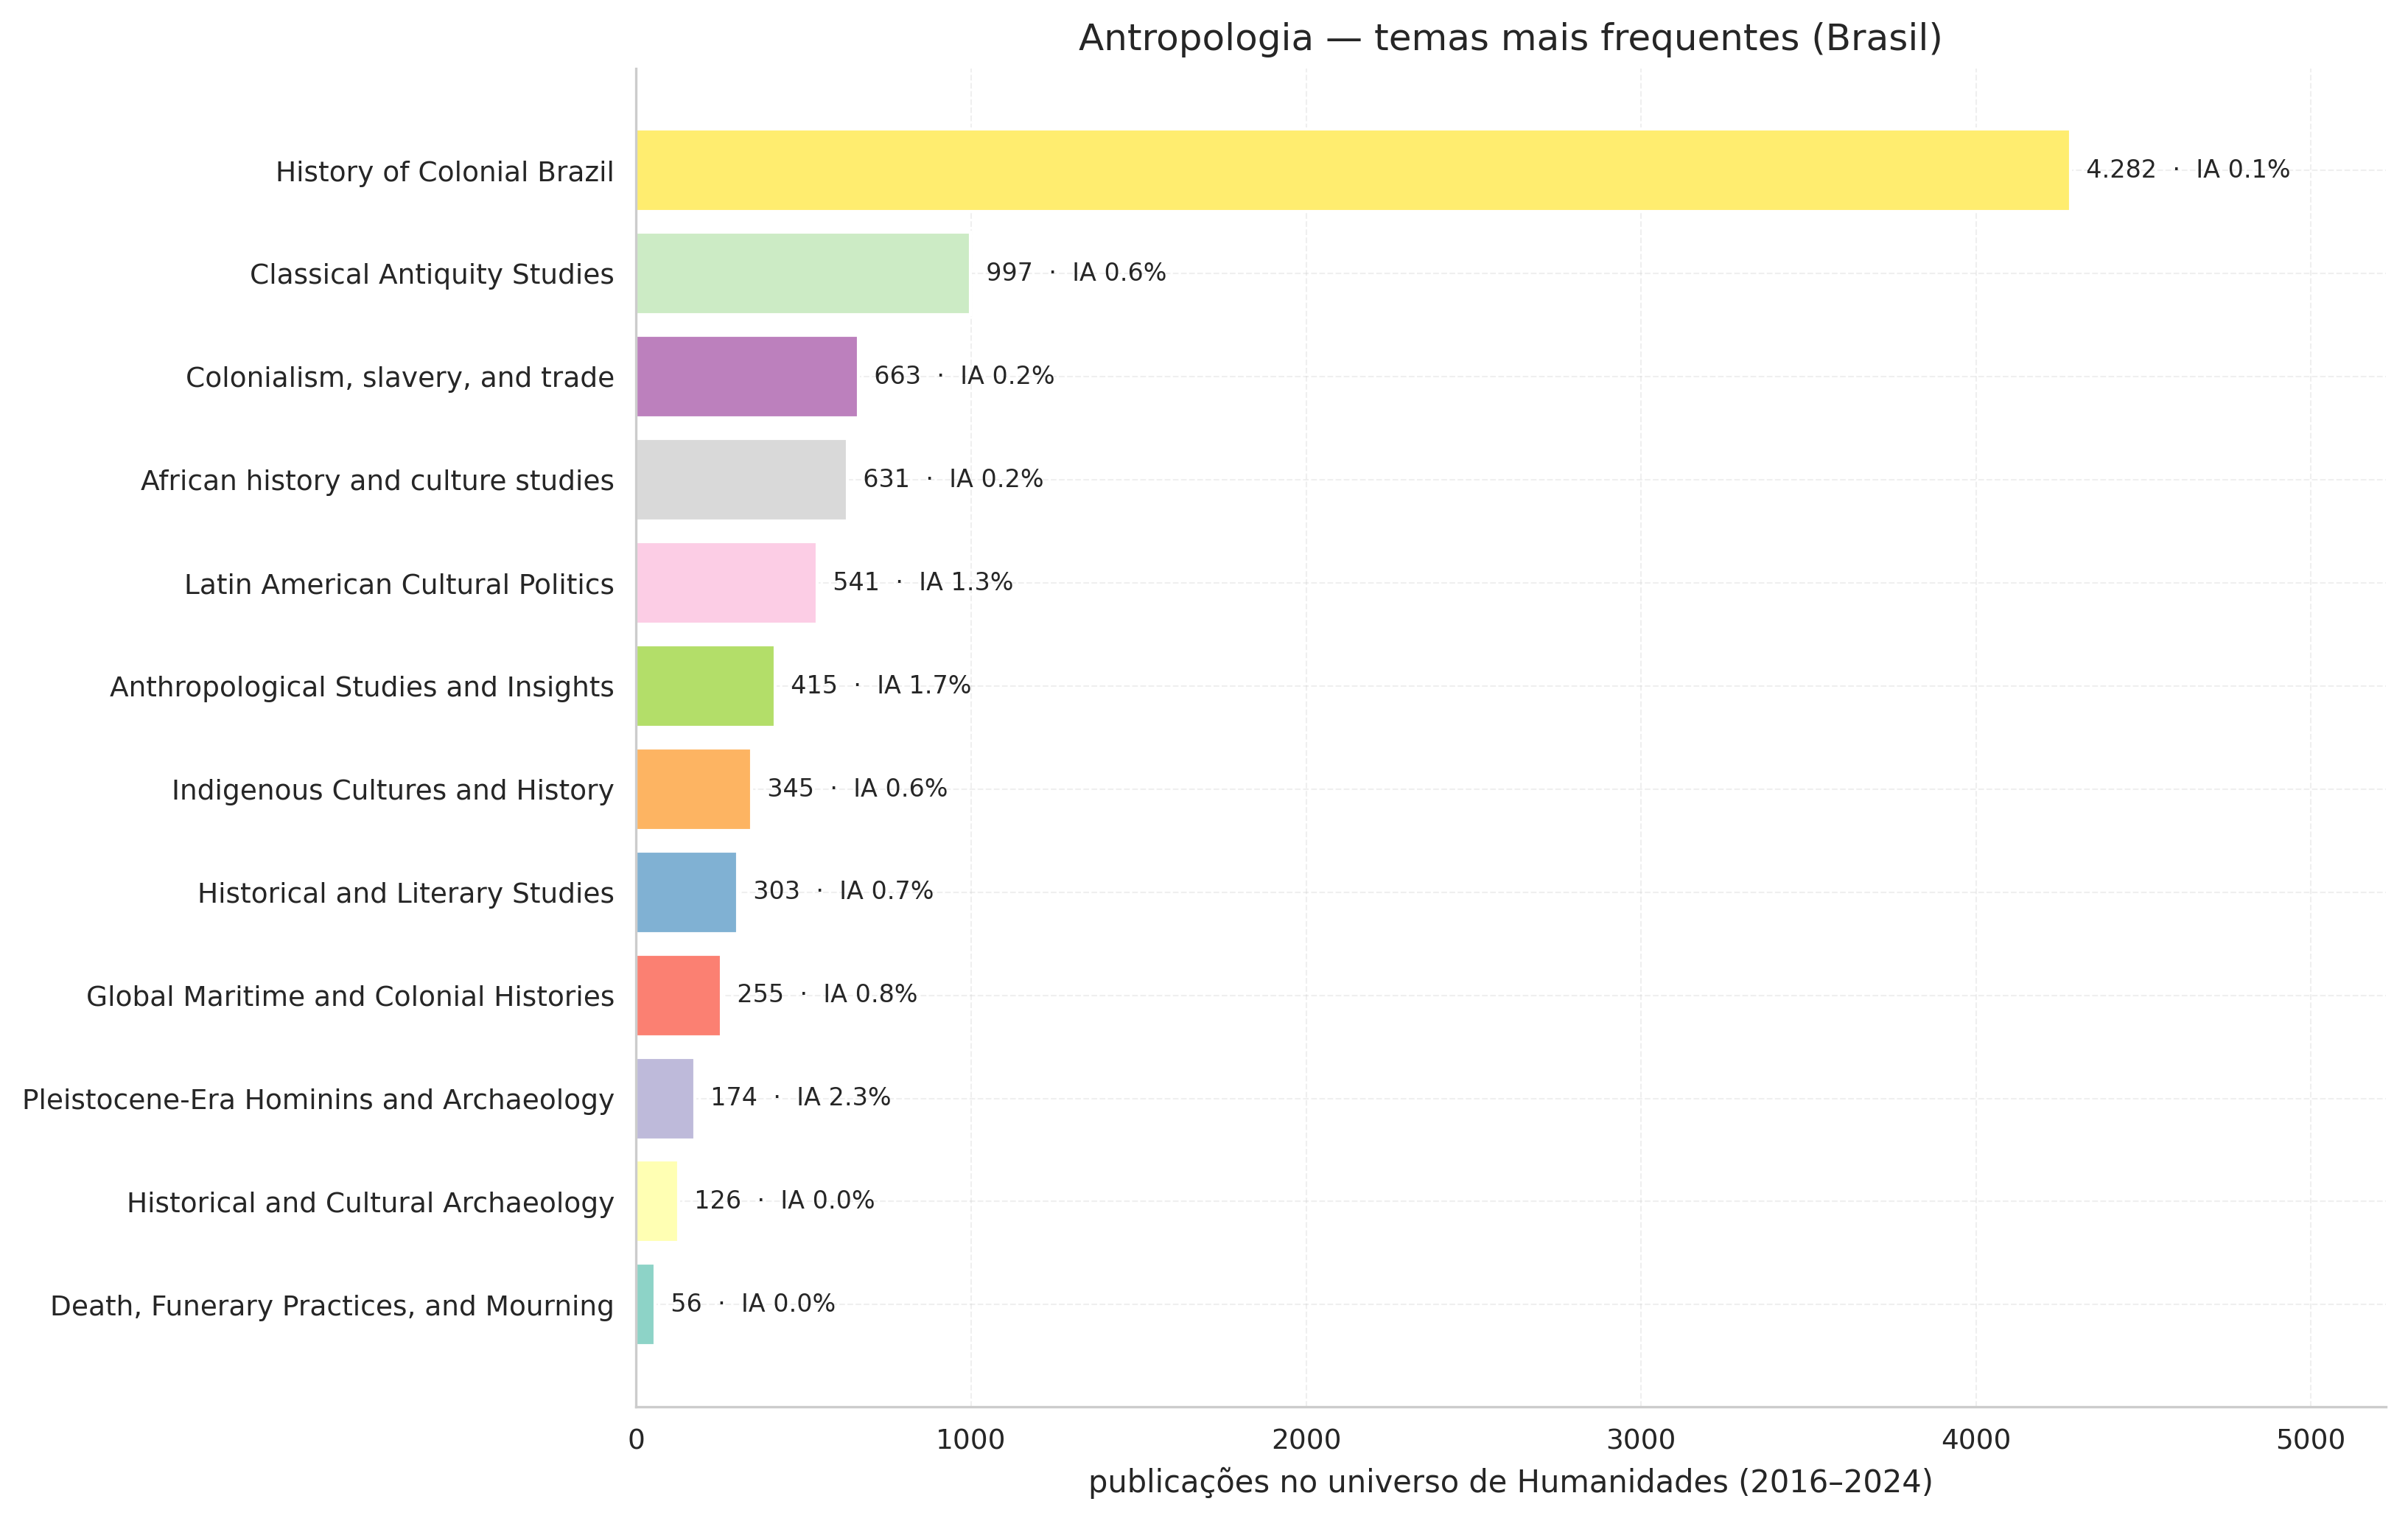
\includegraphics[width=0.85\linewidth]{figuras/openalex_13_anthropology.png}
  \caption{Antropologia (Brasil, 2016--2024): temas (\textit{topics}) mais
  frequentes, com a fração de cada um que toca IA (``IA \%''). O campo é dominado
  por temas histórico-coloniais; a penetração da IA é residual em todos eles.}
  \label{fig:openalex_13_anthropology}
  \fonte{Elaboração própria a partir do OpenAlex (2016--2024).}
\end{figure}

\begin{figure}[htbp]
  \centering
  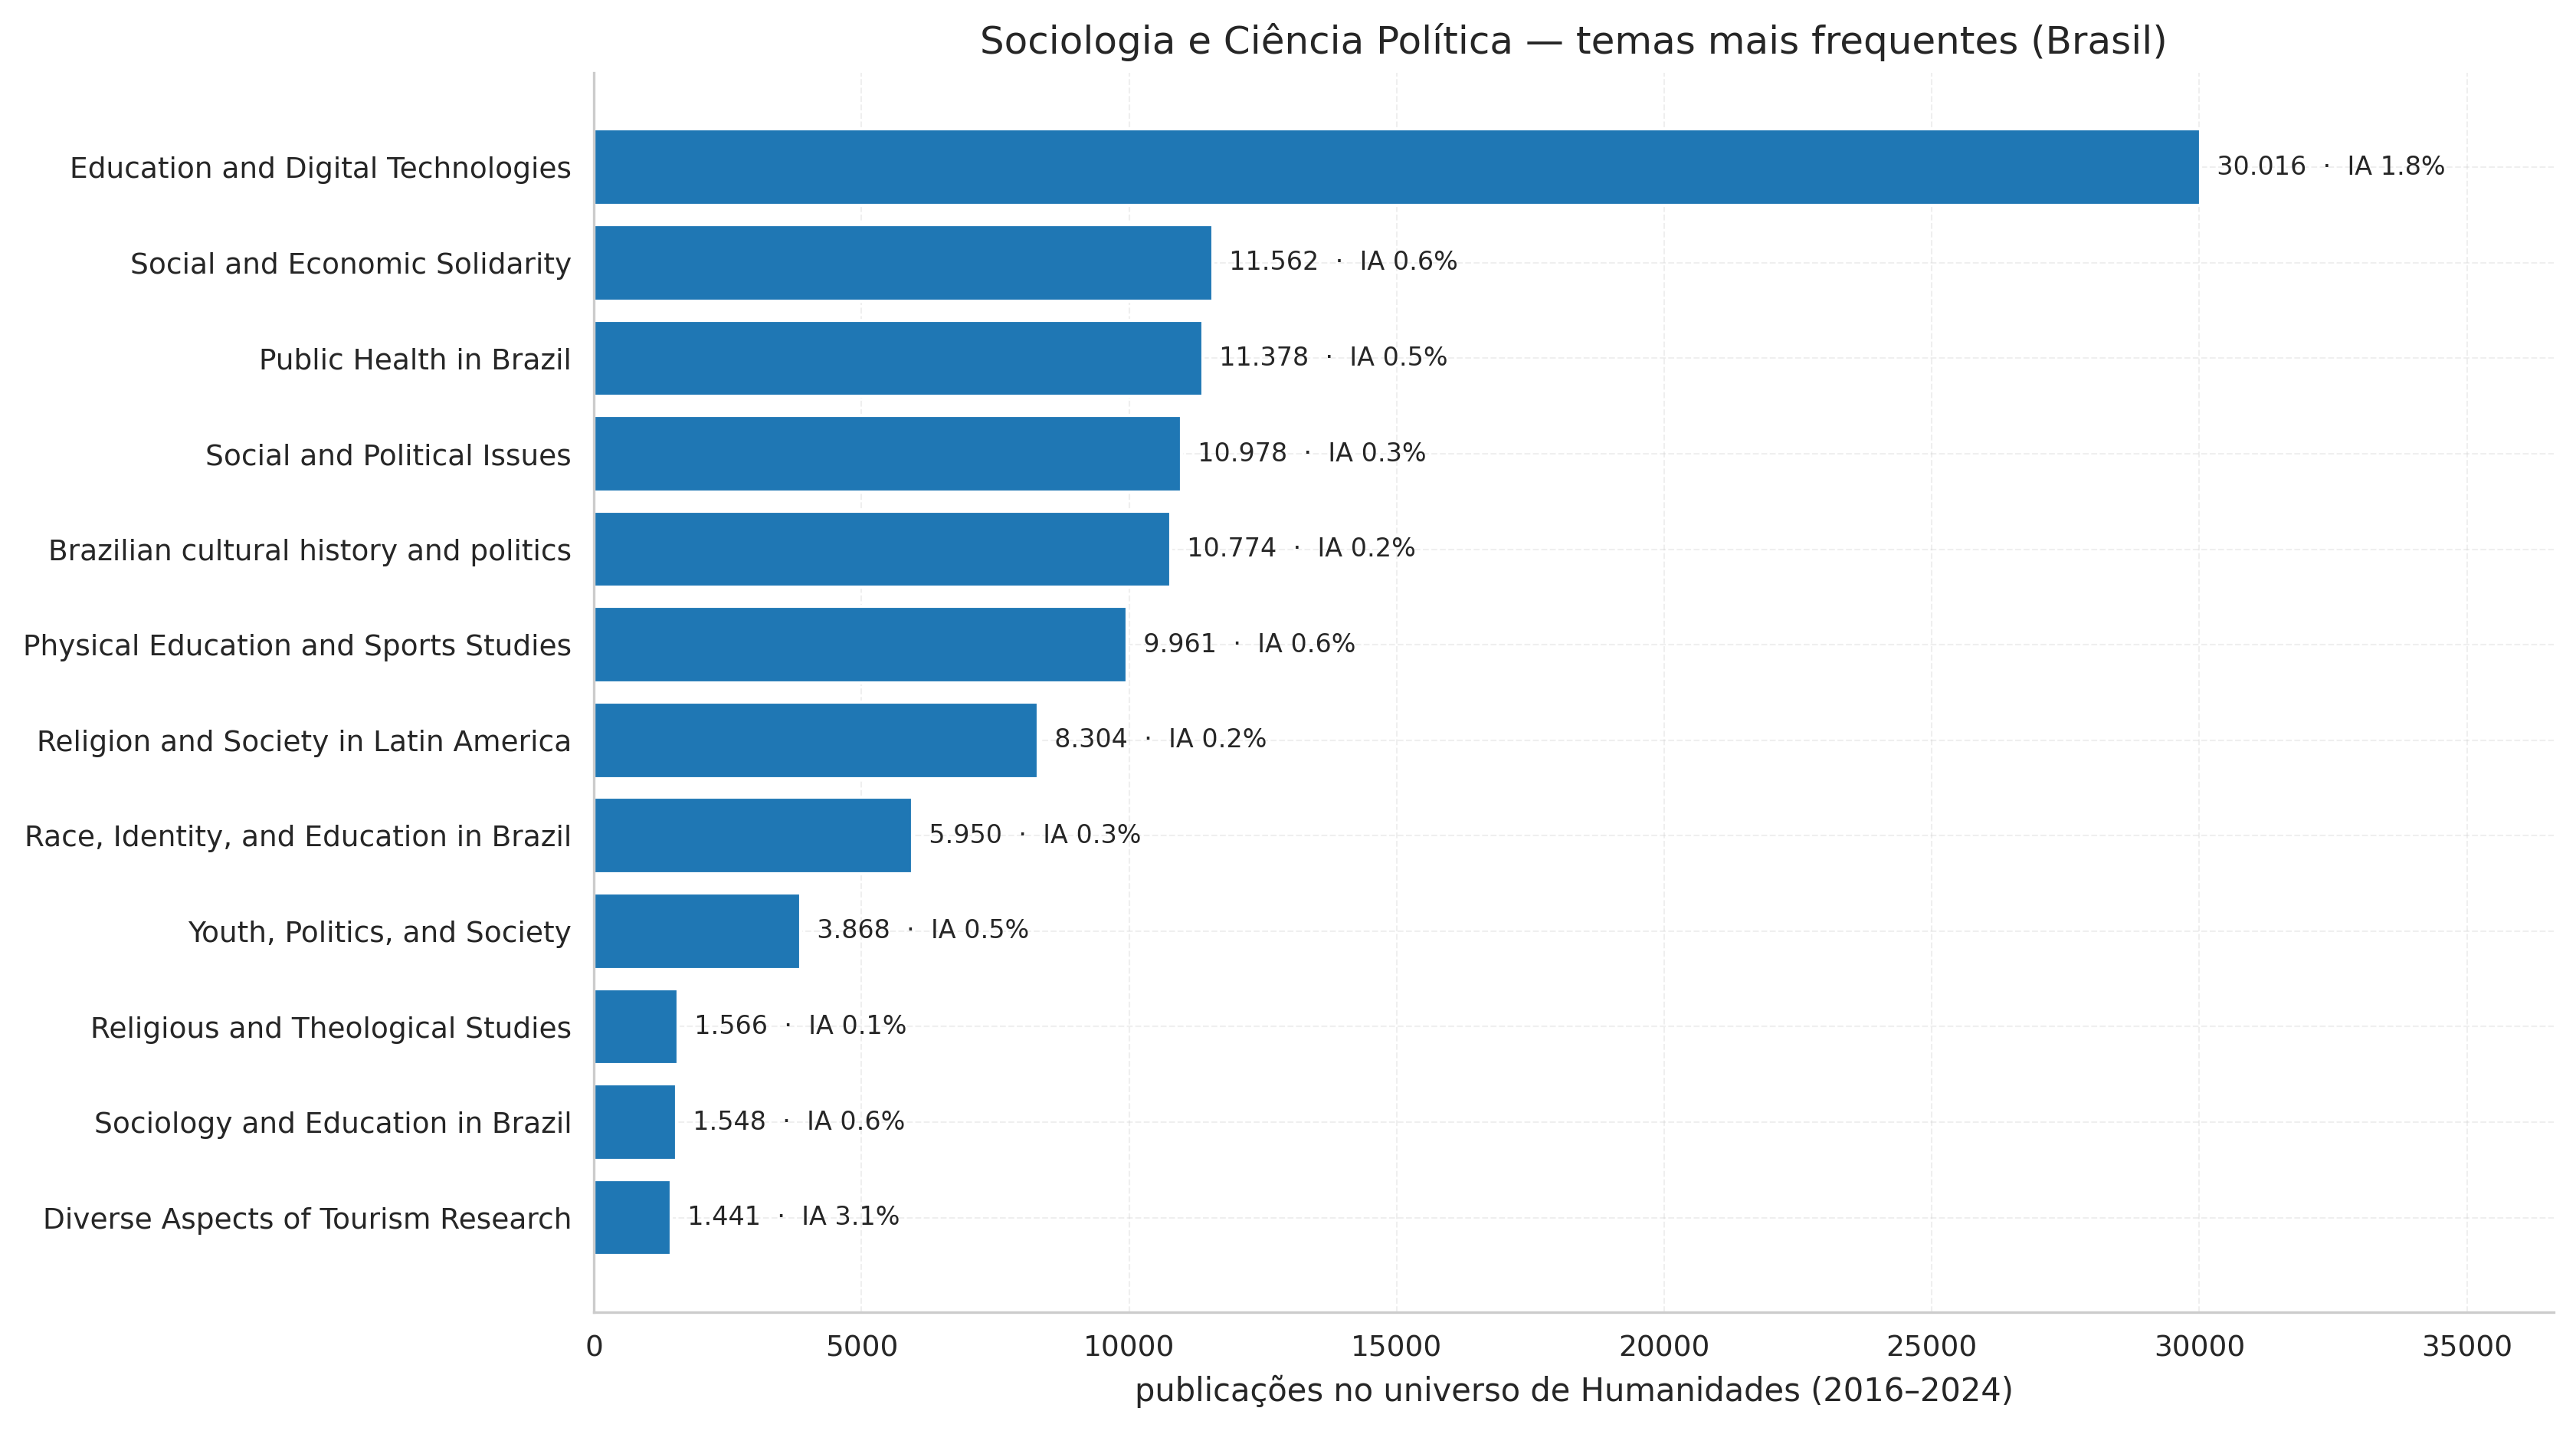
\includegraphics[width=0.85\linewidth]{figuras/openalex_14_sociology_and_political_science.png}
  \caption{Sociologia e Ciência Política (Brasil, 2016--2024): temas mais
  frequentes, com a penetração da IA por tema (``IA \%''). Educação, solidariedade
  social e saúde pública lideram; a IA só se destaca em temas digitais de menor
  volume.}
  \label{fig:openalex_14_sociology}
  \fonte{Elaboração própria a partir do OpenAlex (2016--2024).}
\end{figure}

\begin{figure}[htbp]
  \centering
  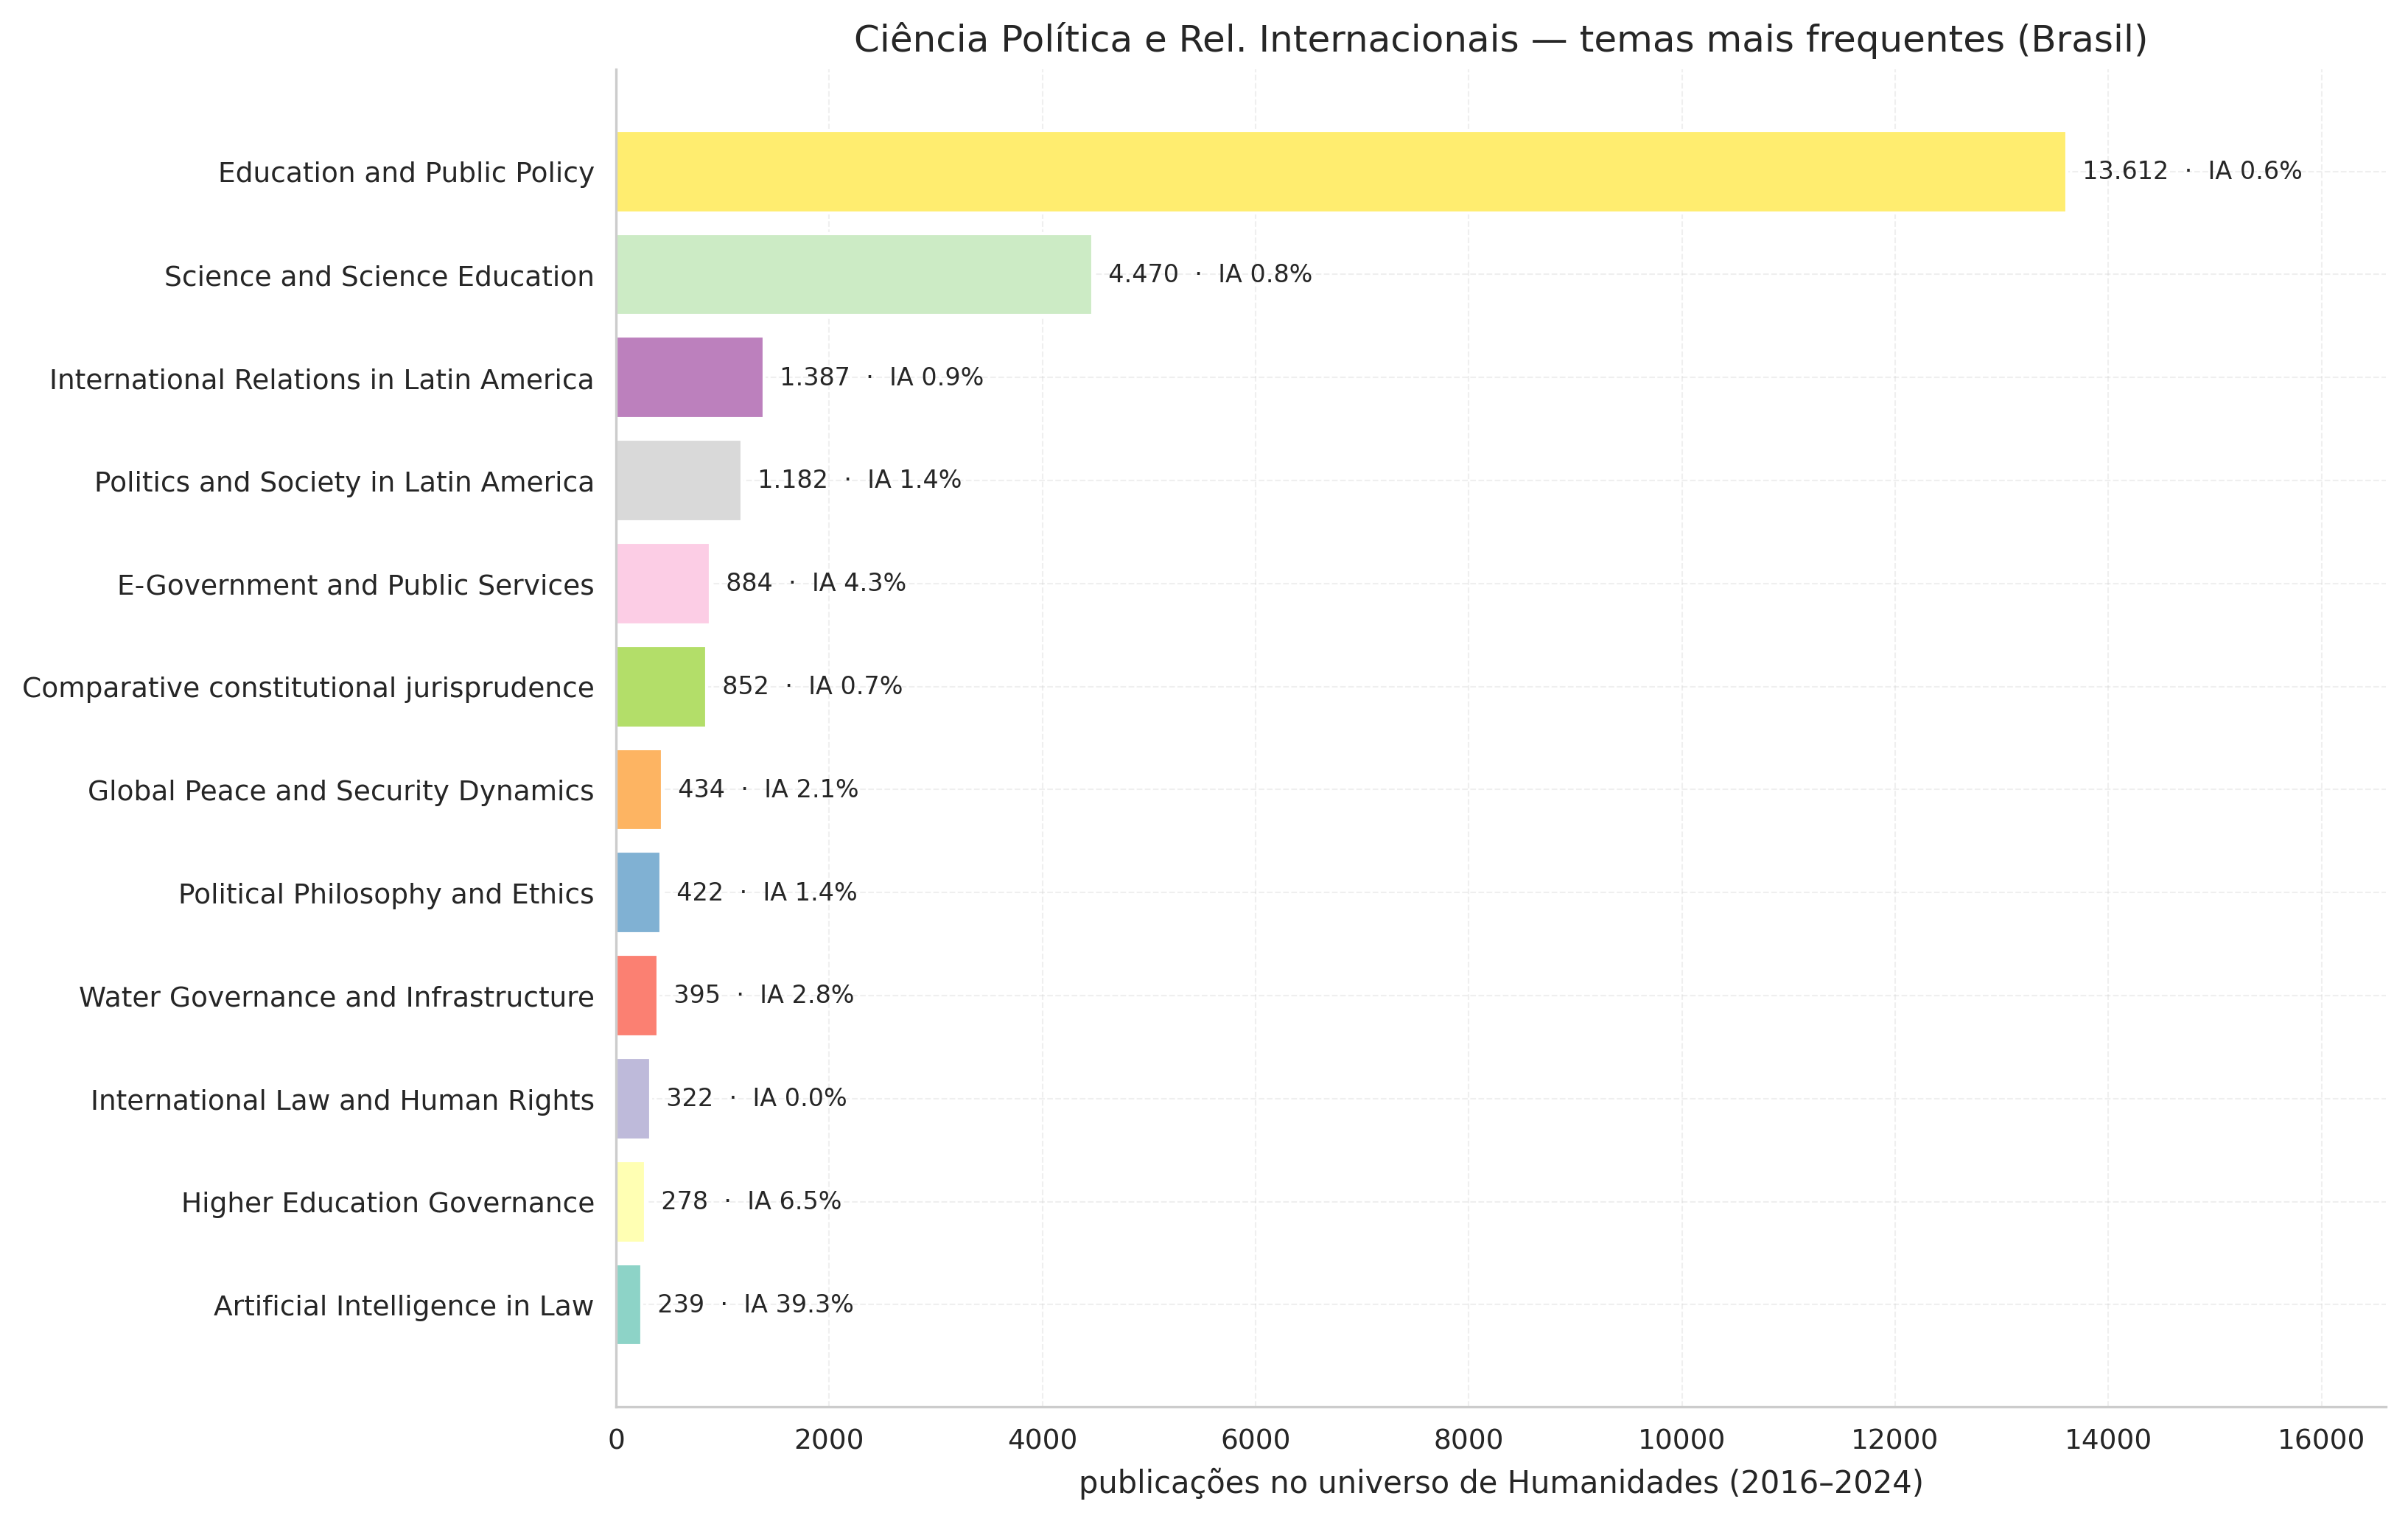
\includegraphics[width=0.85\linewidth]{figuras/openalex_15_political_science_and_international_relations.png}
  \caption{Ciência Política e Relações Internacionais (Brasil, 2016--2024): temas
  mais frequentes, com a penetração da IA por tema (``IA \%''). Educação e
  políticas públicas dominam; ``Artificial Intelligence in Law'' alcança alta
  penetração, mas é tema de pequeno volume.}
  \label{fig:openalex_15_political_science}
  \fonte{Elaboração própria a partir do OpenAlex (2016--2024).}
\end{figure}

\paragraph{Implicação.} O exame temático reforça que a marginalidade da IA não é
um problema de escassez, mas de \emph{natureza dos objetos}: o Brasil pesquisa,
sobretudo, educação, sociedade, história colonial e cultura --- questões de
tradição interpretativa, crítica e qualitativa, que (ainda) não se formulam por
meios computacionais. A IA comparece apenas onde o próprio objeto já é digital.
